\documentclass[11pt]{article}
\usepackage[T1]{fontenc}
\usepackage{lmodern}
\usepackage[a4paper,margin=1in]{geometry}
\usepackage{amsmath,amssymb,amsthm}
\usepackage{booktabs,tabularx,array}
\usepackage{enumitem}
\usepackage{microtype}
\usepackage[round,authoryear]{natbib}
\usepackage[font=small,labelfont=bf]{caption}
\usepackage{xcolor}
\usepackage{pgfplots}
\pgfplotsset{compat=1.18}
\usepgfplotslibrary{groupplots}
\usetikzlibrary{arrows.meta}
\usepackage{hyperref}
\hypersetup{colorlinks=true,linkcolor=blue!60!black,citecolor=blue!60!black,urlcolor=blue!60!black}

\definecolor{cL}{HTML}{0072B2}
\definecolor{cH}{HTML}{D55E00}
\definecolor{cC}{HTML}{009E73}
\definecolor{cA}{HTML}{56B4E9}
\definecolor{cD}{HTML}{E69F00}
\definecolor{cB}{HTML}{CC79A7}

\theoremstyle{plain}
\newtheorem{proposition}{Proposition}
\newtheorem{lemma}{Lemma}
\newtheorem{corollary}{Corollary}
\theoremstyle{definition}
\newtheorem{definition}{Definition}
\newtheorem{assumption}{Assumption}
\newtheorem{remark}{Remark}

\newcommand{\Rcap}{R_{\mathrm{cap}}}
\newcommand{\Vmin}{V_{\min}}
\newcommand{\Valarm}{V_{\mathrm{alarm}}}
\newcommand{\Veff}{V^{\mathrm{eff}}}
\newcommand{\qmax}{q_{\max}}
\newcommand{\dd}{\mathrm{d}}
\newcommand{\spr}{\operatorname{spr}}
\newcommand{\TV}{\operatorname{TV}}
\newcommand{\logit}{\operatorname{logit}}

\title{When Capability Outruns Correction:\\Recursive Capture, Epistemic Lag, and the Case for a Conditional Pause in Frontier AI}
\author{Yongxu Ren\\Independent Researcher}
\date{Second draft for author review --- 29 September 2026}

\begin{document}
\maketitle

\begin{abstract}
The case for slowing frontier artificial intelligence is usually presented as a forecast of catastrophe. This paper argues from correctability instead: whether institutions can detect a failure and change course before its consequences become irreversible. A minimal dynamical theory couples three mechanisms. In \emph{recursive capture}, success converts into rule support that favors the practice that succeeded; above a threshold $\Rcap$ the system is bistable, and inherited rules as well as present shares decide its fate. In \emph{epistemic lag}, evidence about some hazard classes arrives only through exposure, after manifestation windows that no investment in testing shortens; this yields a speed limit on the challenge that assurance must meet, independent of the resources devoted to assurance. In \emph{capture of the evidence channel}, the rules a practice has shaped also shape what is observed about it, which acts as added delay. Coupling the three shows that reforms with the same long-run effect differ in whether the transition crosses a functional floor, because reversal time depends on where a lever acts; that a pause which freezes market shares can complete capture as well as undo it, unless rule-making is insulated while it lasts; and that restraint by a coalition can unwind capture without any agreement, but the coalition required grows as rule support accumulates. The policy implications are a conditional pause on specified frontier transitions, triggered by the absence of a passing independent safety case; paced, bounded exposure where evidence is incompressible; and structural separation of success from rule-setting, applied to the pause regime itself. Each claim is paired with observations that would refute it.
\end{abstract}

\noindent\textbf{Keywords:} AI governance; frontier AI; recursive capture; path dependence; irreversibility; precaution; safety cases; institutional design; dynamical systems.

\section{Introduction}\label{sec:intro}

Increasingly capable AI systems offer real benefits, among them scientific assistance, accessibility and better public services. They also carry substantial uncertainty about our ability to anticipate their behavior, prevent misuse and govern deployment at scale. The \emph{International AI Safety Report 2026} surveys both without converting the evidence into a single uncontested timeline or probability of catastrophe \citep{iasr2026}. Much public argument about slowing frontier development nevertheless turns on exactly such a forecast: advocates of restraint predict disaster, and skeptics dispute the prediction.

This paper starts from a different question. It does not ask whether catastrophe is likely. It asks whether the institutions that choose, evaluate and deploy increasingly capable systems can still detect important failures and change course before the consequences of a wrong decision become irreversible. Call this property \emph{correctability}. The case for restraint is strongest when three conditions hold together:
\begin{enumerate}[label=(\roman*)]
\item the challenge that assurance must meet grows faster than independent assurance and the capacity to respond;
\item competitive and institutional feedback rewards taking that gap, and converts the reward into influence over the rules that measure it;
\item some consequences cannot be repaired once they are detected.
\end{enumerate}
Each condition is empirical, specific to a class of hazards, and subject to change.

The paper develops a minimal dynamical theory of these conditions and of their interaction, and derives a governance design from it. It makes five contributions.
\begin{enumerate}[leftmargin=*]
\item A model of \emph{recursive capture}, in which success converts into rule support that favors the successful practice (Section~\ref{sec:capture}). It has two thresholds: $\Rcap>1$ makes capture possible, and $\Rcap>2$ makes it the long-run convention under small persistent shocks. Its invariant regions show when inherited rules and present shares agree about the outcome and when they conflict.
\item A separation of capture from harm, and a lever-dependent account of reversal (Section~\ref{sec:substrate}). Reforms with identical long-run effects differ in whether the transition crosses a functional floor. As institutions become slow relative to selection, reforms that act on the flow or the decay of rules lose the ability to protect a floor, while reforms that act on the current margin of selection keep it.
\item A decomposition of assurance into compressible and incompressible evidence (Section~\ref{sec:lag}). For incompressible hazard classes it yields a speed limit that no investment in assurance removes. It also classifies hazard classes by whether their manifestation window exceeds their irreversibility horizon.
\item A coupling of capture to observability (Section~\ref{sec:observability}). When evidence arrives through deployment, the deployer's rule support shapes the observation map. Capture then lowers the effective alarm threshold and consumes the correction budget from both ends.
\item An analysis of restraint and of pauses (Section~\ref{sec:pause}). It reconciles unilateral restraint with reciprocal agreement through basin geometry. It also shows what a pause does: it resets rule support to the level that the frozen shares justify under whatever rule-making continues during the pause.
\end{enumerate}
From these follow a decision rule (Section~\ref{sec:decision}), a comparison of three hazard domains (Section~\ref{sec:domains}), a regime design (Section~\ref{sec:regime}) and discriminating tests (Section~\ref{sec:tests}).

\paragraph{Scope and status.} The argument concerns the frontier layer: transitions in the capability and exposure of the most capable systems. It does not assess the wider question of AI's role in competitive and concentrating activities generally. The mechanisms bear on that question, but the argument is not made here, and the restriction of scope implies no judgement about other uses. The formal results are possibility and conditional results about stated models. They are not estimates of present risk, and no parameter is calibrated. Their purpose is to make explicit which empirical quantities decide the policy question, and how. The argument for collective action rests on three further premises, which are normative:
\begin{itemize}[leftmargin=*]
\item severe irreversible harm deserves special weight;
\item independent scrutiny is valuable as a condition of correction;
\item people affected by an optimization process should retain a meaningful capacity to contest its direction.
\end{itemize}

\section{Related work and contribution}\label{sec:related}

\paragraph{Correction and pace.} Collingridge's dilemma states the problem this paper formalizes. While a technology is young it is easy to change, but its effects are unknown; once its effects are known, it is entrenched \citep{collingridge1980}. The law-and-technology literature calls the widening gap between technological change and legal-ethical oversight the \emph{pacing problem} \citep{marchant2011}. Its sociological ancestor is Ogburn's cultural lag \citep{ogburn1922}. On the control side, the requisite-variety and good-regulator results bound what a regulator can correct \citep{ashby1956,conant1970}. Work on resilience and on normal accidents describes how tight coupling and irreversibility turn errors into catastrophes \citep{holling1973,perrow1984}. This paper adds two things: a dynamical account of how entrenchment is produced, and a decomposition of the information side of the dilemma. Together they specify when the dilemma binds.

\paragraph{Races and capture.} Models of AI development races show how competition can erode safety investment and how incentives modify that result, including the risk that blunt regulation suppresses beneficial innovation \citep{armstrong2016,han2021,cimpeanu2022}. \citet{hendrycks2023} argues that selection among AI systems and organizations can favor undesirable traits.

The mechanism of Section~\ref{sec:capture} has precedents:
\begin{itemize}[leftmargin=*]
\item regulatory capture \citep{stigler1971,dalbo2006,carpenter2013};
\item increasing returns and path dependence in technologies and institutions \citep{david1985,arthur1989,pierson2000};
\item niche construction, in which organisms modify the environment that selects them \citep{odlingsmee2003};
\item evolutionary games with environmental feedback \citep{weitz2016,tilman2020}.
\end{itemize}

Structural and accumulative accounts of AI risk hold that harm can arise from incentives and interaction without any single failure or malicious actor \citep{zwetsloot2019,critch2023,kasirzadeh2025,kulveit2025}. Here, ``capture'' means a practice's influence over the conditions of its own future selection. That includes regulatory capture but is broader: benchmark design, procurement defaults, evaluation conventions and standards of care all belong to the rule environment.

\paragraph{Governance instruments.} Much of what Section~\ref{sec:regime} proposes already exists in some form:
\begin{itemize}[leftmargin=*]
\item \emph{Developer commitments:} responsible scaling policies and if-then commitments \citep{anthropic2023,karnofsky2024}. In the Frontier AI Safety Commitments, signatories undertook, in the extreme, not to develop or deploy a model if mitigations cannot keep risk below their thresholds \citep{seoul2024}.
\item \emph{Evaluation-based coordination:} coordinated pausing among developers \citep{alaga2023}, safety cases \citep{clymer2024,buhl2024}, dangerous-capability evaluations \citep{shevlane2023} and frontier regulation \citep{anderljung2023}.
\item \emph{Compute governance and verification} \citep{shavit2023,sastry2024,wasil2024,baker2025}, together with the limits of compute thresholds \citep{hooker2024}.
\item \emph{Statute:} the EU AI Act and California's Transparency in Frontier Artificial Intelligence Act \citep{euaiact2024,sb53}.
\item \emph{Calls for a pause} \citep{fli2023}, and scientists' consensus statements proposing red lines \citep{idais2024}.
\end{itemize}
These regimes largely share one feature: thresholds and evaluations are set or assessed by the developers whose transitions they govern. The capture model explains why that feature is fragile, and what a regime must do about it.

\paragraph{Precaution and option value.} Two strands support the decision rule of Section~\ref{sec:decision}: maxmin expected utility under ambiguity \citep{gilboa1989}, and the value of preserving flexibility under irreversibility and learning \citep{arrowfisher1974,henry1974,dixitpindyck1994,gollier2000}. Its critics and its fat-tailed variants mark the rule's limits \citep{sunstein2005,weitzman2009,taleb2014}.

\paragraph{Contribution.} Each mechanism studied here has precedents, and the contribution lies in coupling them in one model. The coupling yields four results that the separate literatures do not supply. Reversal latency depends on the lever. Incompressible evidence imposes a speed limit that assurance investment cannot lift. Capture of the evidence channel acts as delay. And a pause resets rule support to the level that frozen shares justify, which can complete capture as well as undo it.

\section{Recursive capture}\label{sec:capture}

\subsection{A minimal model}

Consider a population of development and deployment decisions. A share $x\in[0,1]$ follows a practice $E$, and the rest follow an alternative practice $E'$. Let $r\ge 0$ measure \emph{rule support}: the extent to which the environment that selects among practices favors $E$. The dynamics are
\begin{equation}\label{eq:core}
\dot x=\kappa\, x(1-x)(ar-c),\qquad \dot r=\varepsilon\,(bx-dr),
\end{equation}
with $a,b,c,d,\kappa,\varepsilon>0$. The first equation is replicator dynamics on relative payoff \citep{hofbauer1998}. Under neutral rules, $E$ carries a net relative cost $c$. Rule support offsets that cost at rate $a$. The second equation converts adoption into rule support at rate $b$, and rule support decays or is corrected at rate $d$. Rules typically change more slowly than practice ($\varepsilon<\kappa$).

For frontier AI, one reading takes $E$ to be releasing or scaling systems before independent evaluation has concluded. Then $r$ is the extent to which evaluation conventions, benchmark suites, procurement criteria and standards of care are defined by reference to what deployed systems already do. Under neutral rules, early release costs more than it gains: it brings liability exposure, lost trust and the expense of later correction. Once the rules take their reference from deployed systems, that cost is offset:
\begin{itemize}[leftmargin=*]
\item benchmarks are built from deployed systems;
\item procurement requires compatibility with incumbent interfaces;
\item prevailing practice sets the standard of care.
\end{itemize}
The conversion need not be deliberate. Trained staff, standard interfaces, dependencies and ordinary procurement preserve it.

Other readings are possible, since $E$ could be a training practice, a deployment architecture or an organizational form. The analysis needs only that success feed back into the conditions of future selection. If $c\le 0$, the practice wins under neutral rules and needs no capture to spread. That case is a social dilemma, treated in Section~\ref{sec:pause}. The model isolates the case in which a practice that would lose under neutral rules comes to dominate because of rules it helped to shape. This is the case in which reform is expected to work, and may not.

\begin{definition}[Recursive capture]\label{def:capture}
A system exhibits \emph{recursive capture} when present success of a practice increases its influence on the conditions of future selection, and that influence increases the relative success of the practice. The captured state is called an attractor only once an attracting region has been established. Persistence of a practice does not by itself establish one.
\end{definition}

Let $\Rcap=ab/(cd)$. It compares the rule support generated at full adoption, $b/d$, weighted by its effect $a$, with the cost $c$ that support must overcome.

\begin{proposition}[Thresholds, bistability and structure]\label{prop:capture}
\begin{enumerate}[label=(\roman*),leftmargin=*]
\item If $\Rcap<1$, every solution with $x(0)\in[0,1)$ converges to $L=(0,0)$.
\item If $\Rcap>1$, the equilibria are $L$, $H=(1,b/d)$ and $S=(1/\Rcap,\,c/a)$. $L$ and $H$ are locally asymptotically stable, $S$ is a saddle, and every solution converges to one of the three. The stable manifold of $S$ is the graph of a nonincreasing function $x=\sigma(r)$ on $[0,\infty)$, with $\sigma(c/a)=1/\Rcap$, $1/\Rcap<\sigma(0)<1$ and $\sigma(r)\to0$ as $r\to\infty$. It separates the basin of $L$ (below it) from that of $H$ (above it).
\item The flow is gradient-like for $\Phi(x,r)=axr-cx-\tfrac{ad}{2b}r^2$: $\dot x=\kappa x(1-x)\,\partial_x\Phi$ and $\dot r=(\varepsilon b/a)\,\partial_r\Phi$, so that $\Phi$ is nondecreasing along solutions and strictly increasing except at equilibria.
\item The open quadrants $Q_L=\{x<1/\Rcap,\ r<c/a\}$ and $Q_H=\{x>1/\Rcap,\ r>c/a\}$ are forward invariant and lie in the basins of $L$ and $H$ respectively.
\end{enumerate}
\end{proposition}

All proofs are in Appendix~\ref{app:proofs}. Part (iv) says when the outcome is settled: when present share and inherited rule support are both below their saddle values, or both above them. Where they disagree, a large share under weak rules or a small share under strong rules, the separatrix decides, and its position depends on the relative speed of rules and selection.

\begin{remark}[Which clock decides]\label{rem:clocks}
As $\varepsilon/\kappa\to0$ (rules slow relative to selection), the separatrix approaches the line $r=c/a$, so inherited rules decide the outcome. As $\varepsilon/\kappa\to\infty$ it approaches $x=1/\Rcap$, so present shares decide. Standards, procurement rules and doctrines of liability change more slowly than market shares, which places frontier AI governance nearer the first regime.
\end{remark}

\begin{remark}[A second threshold]\label{rem:riskdominance}
In the fast-rule reduction $r=bx/d$, the relative payoff of $E$ is $c(\Rcap x-1)$, which increases with $x$. Rule memory therefore creates positive frequency dependence, and both conventions are equilibria of a coordination game. The capture equilibrium is risk-dominant exactly when $\Rcap>2$, which is also when $\Phi(H)>\Phi(L)=0$. Under stochastic evolutionary dynamics with small persistent shocks, the risk-dominant convention is selected in the long run \citep{kandori1993,young1993}. Hence $\Rcap>1$ makes capture possible, and $\Rcap>2$ makes it the convention that noise eventually selects.
\end{remark}

\begin{corollary}[Path dependence]\label{cor:path}
If $\Rcap>1$, two systems with the same present share can have different fates if they inherit different rule support. Replacing the leaders or the models of a captured practice need not replace the selection environment that promoted them.
\end{corollary}

\begin{figure}[t]
\centering
% --- figure generated by figures.py (fig-phase.tex) ---
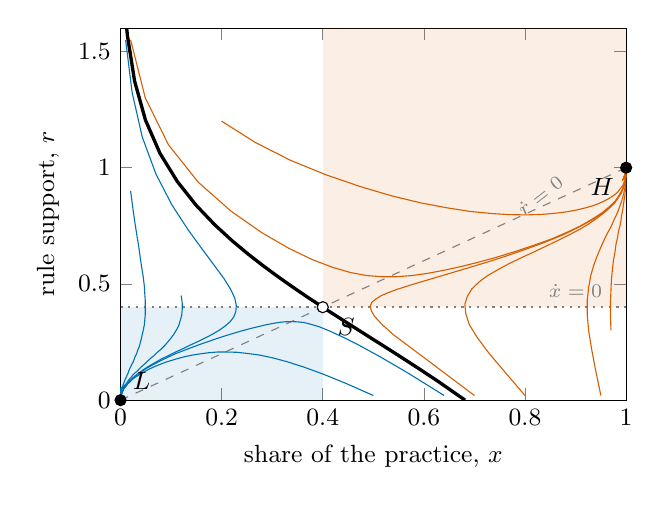
\begin{tikzpicture}
\begin{axis}[width=0.66\linewidth, height=0.52\linewidth, xmin=0, xmax=1, ymin=0, ymax=1.6,
  xlabel={share of the practice, $x$}, ylabel={rule support, $r$}, tick label style={font=\small},
  label style={font=\small}, clip=true]
\fill[cL, opacity=0.10] (axis cs:0,0) rectangle (axis cs:0.4,0.4);
\fill[cH, opacity=0.10] (axis cs:0.4,0.4) rectangle (axis cs:1,1.6);
\addplot[gray, dashed, domain=0:1, samples=2] {x};
\addplot[gray, dotted, thick, domain=0:1, samples=2] {0.4};
\addplot[cH, thin, -{Stealth[length=4pt]}] coordinates {(0.950,0.020) (0.940,0.125) (0.932,0.216) (0.926,0.297) (0.923,0.368) (0.923,0.431) (0.926,0.486) (0.930,0.536) (0.936,0.581) (0.943,0.622) (0.950,0.658) (0.957,0.692) (0.964,0.722) (0.971,0.750) (0.976,0.775) (0.981,0.798) (0.985,0.819) (0.988,0.838) (0.991,0.855) (0.993,0.871) (0.995,0.885) (0.996,0.897) (0.997,0.909) (0.998,0.919) (0.999,0.928) (0.999,0.936) (0.999,0.943) (0.999,0.949) (1.000,0.955) (1.000,0.960) (1.000,0.964) (1.000,0.968) (1.000,0.972) (1.000,0.975) (1.000,0.978) (1.000,0.980) (1.000,0.983) (1.000,0.985) (1.000,0.986) (1.000,0.988) (1.000,0.989) (1.000,0.990)};
\addplot[cH, thin, -{Stealth[length=4pt]}] coordinates {(0.800,0.020) (0.761,0.119) (0.729,0.201) (0.706,0.268) (0.690,0.324) (0.683,0.371) (0.681,0.412) (0.686,0.447) (0.695,0.479) (0.709,0.508) (0.726,0.536) (0.747,0.562) (0.769,0.588) (0.793,0.613) (0.818,0.638) (0.842,0.663) (0.866,0.688) (0.889,0.713) (0.910,0.737) (0.928,0.761) (0.943,0.784) (0.956,0.806) (0.967,0.826) (0.976,0.845) (0.982,0.863) (0.987,0.879) (0.991,0.893) (0.993,0.906) (0.995,0.918) (0.997,0.928) (0.998,0.937) (0.998,0.945) (0.999,0.952) (0.999,0.958) (1.000,0.964) (1.000,0.968) (1.000,0.972) (1.000,0.976) (1.000,0.979) (1.000,0.982) (1.000,0.984) (1.000,0.986) (1.000,0.988) (1.000,0.990) (1.000,0.990)};
\addplot[cH, thin, -{Stealth[length=4pt]}] coordinates {(0.700,0.020) (0.629,0.136) (0.577,0.221) (0.540,0.281) (0.517,0.326) (0.503,0.359) (0.496,0.384) (0.494,0.404) (0.497,0.421) (0.505,0.435) (0.515,0.449) (0.529,0.462) (0.546,0.476) (0.566,0.490) (0.590,0.506) (0.618,0.524) (0.649,0.544) (0.683,0.566) (0.721,0.591) (0.760,0.618) (0.800,0.648) (0.839,0.679) (0.875,0.711) (0.906,0.744) (0.933,0.776) (0.954,0.806) (0.969,0.835) (0.980,0.860) (0.987,0.883) (0.992,0.902) (0.995,0.919) (0.997,0.933) (0.998,0.945) (0.999,0.954) (0.999,0.963) (1.000,0.969) (1.000,0.975) (1.000,0.979) (1.000,0.983) (1.000,0.986) (1.000,0.989) (1.000,0.990)};
\addplot[cL, thin, -{Stealth[length=4pt]}] coordinates {(0.640,0.020) (0.569,0.116) (0.514,0.186) (0.472,0.236) (0.439,0.272) (0.414,0.297) (0.394,0.315) (0.377,0.326) (0.363,0.334) (0.349,0.337) (0.337,0.338) (0.324,0.337) (0.312,0.334) (0.299,0.329) (0.285,0.323) (0.270,0.315) (0.255,0.307) (0.238,0.297) (0.221,0.286) (0.203,0.274) (0.184,0.260) (0.165,0.246) (0.146,0.231) (0.128,0.216) (0.109,0.200) (0.092,0.183) (0.077,0.167) (0.063,0.151) (0.050,0.135) (0.040,0.120) (0.031,0.106) (0.024,0.093) (0.018,0.081) (0.014,0.071) (0.010,0.061) (0.007,0.052) (0.005,0.045) (0.004,0.038) (0.003,0.032) (0.002,0.027) (0.001,0.023) (0.001,0.020) (0.001,0.019)};
\addplot[cL, thin, -{Stealth[length=4pt]}] coordinates {(0.500,0.020) (0.447,0.071) (0.402,0.111) (0.363,0.142) (0.330,0.165) (0.301,0.182) (0.275,0.194) (0.251,0.201) (0.230,0.206) (0.210,0.207) (0.191,0.207) (0.174,0.204) (0.157,0.199) (0.142,0.194) (0.127,0.187) (0.113,0.179) (0.101,0.171) (0.089,0.163) (0.078,0.154) (0.067,0.144) (0.058,0.135) (0.050,0.126) (0.043,0.117) (0.036,0.108) (0.030,0.100) (0.025,0.092) (0.021,0.084) (0.018,0.077) (0.014,0.070) (0.012,0.063) (0.010,0.057) (0.008,0.052) (0.006,0.047) (0.005,0.042) (0.004,0.038) (0.003,0.034) (0.003,0.031) (0.002,0.027) (0.002,0.024) (0.001,0.022) (0.001,0.020) (0.001,0.019)};
\addplot[cH, thin, -{Stealth[length=4pt]}] coordinates {(0.020,1.550) (0.049,1.300) (0.095,1.098) (0.154,0.937) (0.218,0.814) (0.279,0.721) (0.333,0.653) (0.380,0.604) (0.420,0.571) (0.455,0.549) (0.487,0.536) (0.517,0.531) (0.546,0.531) (0.576,0.536) (0.606,0.545) (0.638,0.558) (0.672,0.574) (0.707,0.593) (0.744,0.615) (0.780,0.639) (0.817,0.666) (0.852,0.693) (0.883,0.722) (0.911,0.751) (0.934,0.780) (0.953,0.807) (0.967,0.832) (0.978,0.855) (0.985,0.876) (0.990,0.895) (0.994,0.911) (0.996,0.925) (0.998,0.937) (0.999,0.947) (0.999,0.955) (0.999,0.963) (1.000,0.969) (1.000,0.974) (1.000,0.978) (1.000,0.982) (1.000,0.985) (1.000,0.987) (1.000,0.989) (1.000,0.990)};
\addplot[cL, thin, -{Stealth[length=4pt]}] coordinates {(0.010,1.550) (0.023,1.323) (0.043,1.132) (0.070,0.973) (0.101,0.842) (0.133,0.735) (0.162,0.648) (0.186,0.578) (0.205,0.522) (0.218,0.476) (0.226,0.439) (0.229,0.407) (0.228,0.381) (0.224,0.358) (0.217,0.338) (0.207,0.319) (0.196,0.302) (0.183,0.285) (0.169,0.269) (0.154,0.253) (0.138,0.237) (0.123,0.221) (0.108,0.206) (0.093,0.190) (0.079,0.175) (0.067,0.160) (0.055,0.145) (0.045,0.131) (0.037,0.118) (0.029,0.105) (0.023,0.093) (0.018,0.083) (0.014,0.073) (0.011,0.064) (0.008,0.056) (0.006,0.049) (0.005,0.042) (0.004,0.037) (0.003,0.032) (0.002,0.027) (0.001,0.024) (0.001,0.020) (0.001,0.019)};
\addplot[cH, thin, -{Stealth[length=4pt]}] coordinates {(0.200,1.200) (0.267,1.108) (0.337,1.031) (0.407,0.969) (0.474,0.919) (0.536,0.879) (0.593,0.849) (0.644,0.828) (0.691,0.812) (0.733,0.803) (0.770,0.798) (0.803,0.797) (0.833,0.799) (0.859,0.804) (0.882,0.810) (0.902,0.818) (0.919,0.827) (0.934,0.836) (0.946,0.846) (0.956,0.856) (0.965,0.866) (0.972,0.876) (0.978,0.885) (0.983,0.894) (0.986,0.903) (0.989,0.911) (0.992,0.919) (0.994,0.926) (0.995,0.932) (0.996,0.938) (0.997,0.944) (0.998,0.949) (0.998,0.954) (0.999,0.958) (0.999,0.962) (0.999,0.965) (0.999,0.969) (1.000,0.972) (1.000,0.974) (1.000,0.977) (1.000,0.979) (1.000,0.981) (1.000,0.983) (1.000,0.984) (1.000,0.986) (1.000,0.987) (1.000,0.988) (1.000,0.989) (1.000,0.990)};
\addplot[cL, thin, -{Stealth[length=4pt]}] coordinates {(0.020,0.900) (0.024,0.832) (0.028,0.770) (0.032,0.714) (0.036,0.661) (0.039,0.613) (0.042,0.569) (0.045,0.529) (0.047,0.492) (0.048,0.458) (0.049,0.426) (0.049,0.397) (0.049,0.370) (0.048,0.346) (0.047,0.323) (0.045,0.301) (0.043,0.282) (0.041,0.263) (0.039,0.246) (0.037,0.230) (0.034,0.215) (0.032,0.201) (0.029,0.188) (0.027,0.176) (0.025,0.164) (0.022,0.153) (0.020,0.143) (0.018,0.134) (0.016,0.125) (0.015,0.116) (0.013,0.108) (0.012,0.101) (0.010,0.094) (0.009,0.088) (0.008,0.082) (0.007,0.076) (0.006,0.071) (0.005,0.066) (0.005,0.061) (0.004,0.057) (0.004,0.053) (0.003,0.049) (0.003,0.045) (0.002,0.042) (0.002,0.039) (0.002,0.036) (0.002,0.033) (0.001,0.031) (0.001,0.029) (0.001,0.027) (0.001,0.027)};
\addplot[cH, thin, -{Stealth[length=4pt]}] coordinates {(0.970,0.300) (0.969,0.364) (0.969,0.421) (0.970,0.473) (0.971,0.521) (0.973,0.564) (0.975,0.603) (0.978,0.638) (0.980,0.671) (0.983,0.700) (0.985,0.727) (0.988,0.752) (0.990,0.775) (0.991,0.795) (0.993,0.814) (0.994,0.831) (0.995,0.847) (0.996,0.861) (0.997,0.874) (0.998,0.886) (0.998,0.896) (0.999,0.906) (0.999,0.915) (0.999,0.923) (0.999,0.930) (1.000,0.937) (1.000,0.943) (1.000,0.948) (1.000,0.953) (1.000,0.957) (1.000,0.961) (1.000,0.965) (1.000,0.968) (1.000,0.971) (1.000,0.974) (1.000,0.977) (1.000,0.979) (1.000,0.981) (1.000,0.983) (1.000,0.984) (1.000,0.986) (1.000,0.987) (1.000,0.988) (1.000,0.989) (1.000,0.990)};
\addplot[cL, thin, -{Stealth[length=4pt]}] coordinates {(0.120,0.450) (0.122,0.419) (0.122,0.390) (0.121,0.365) (0.118,0.342) (0.115,0.320) (0.110,0.300) (0.105,0.282) (0.099,0.265) (0.093,0.249) (0.087,0.234) (0.080,0.219) (0.073,0.206) (0.067,0.193) (0.060,0.181) (0.054,0.169) (0.049,0.158) (0.043,0.147) (0.038,0.137) (0.034,0.127) (0.029,0.118) (0.025,0.110) (0.022,0.101) (0.019,0.094) (0.016,0.086) (0.014,0.080) (0.012,0.073) (0.010,0.067) (0.009,0.062) (0.007,0.057) (0.006,0.052) (0.005,0.048) (0.004,0.043) (0.004,0.040) (0.003,0.036) (0.003,0.033) (0.002,0.030) (0.002,0.027) (0.001,0.025) (0.001,0.023) (0.001,0.021)};
\addplot[black, very thick] coordinates {(0.6814,0.0001) (0.6272,0.0822) (0.5816,0.1477) (0.5444,0.1998) (0.5145,0.2411) (0.4906,0.2739) (0.4718,0.2999) (0.4568,0.3205) (0.4450,0.3369) (0.4357,0.3499) (0.4283,0.3602) (0.4225,0.3683) (0.4178,0.3748) (0.4141,0.3800) (0.4112,0.3841) (0.4089,0.3874) (0.4071,0.3899) (0.4056,0.3920) (0.4045,0.3936) (0.4036,0.3949) (0.4028,0.3960) (0.4023,0.3968) (0.4018,0.3975) (0.4014,0.3980) (0.4011,0.3984) (0.4009,0.3987) (0.4007,0.3990) (0.4006,0.3992) (0.4005,0.3994) (0.4004,0.3995) (0.4003,0.3996) (0.4002,0.3997) (0.4002,0.3997) (0.4001,0.3998) (0.4001,0.3998) (0.4001,0.3999) (0.4001,0.3999) (0.4001,0.3999) (0.4000,0.3999) (0.4000,0.3999) (0.4000,0.4000) (0.4000,0.4000) (0.4000,0.4000) (0.4000,0.4000) (0.4000,0.4000) (0.4000,0.4000) (0.4000,0.4000) (0.4000,0.4000) (0.4000,0.4000) (0.4000,0.4000) (0.4000,0.4000) (0.4000,0.4000) (0.4000,0.4000) (0.4000,0.4000) (0.4000,0.4000) (0.4000,0.4000) (0.4000,0.4000) (0.4000,0.4000) (0.4000,0.4000) (0.4000,0.4000) (0.4000,0.4000) (0.4000,0.4000) (0.4000,0.4000) (0.4000,0.4000) (0.4000,0.4000) (0.4000,0.4000) (0.4000,0.4000) (0.4000,0.4000) (0.4000,0.4000) (0.4000,0.4000) (0.4000,0.4000) (0.4000,0.4000) (0.4000,0.4000) (0.4000,0.4000) (0.4000,0.4000) (0.4000,0.4000) (0.4000,0.4001) (0.3999,0.4001) (0.3999,0.4001) (0.3999,0.4001) (0.3999,0.4002) (0.3999,0.4002) (0.3998,0.4002) (0.3998,0.4003) (0.3997,0.4004) (0.3997,0.4005) (0.3996,0.4006) (0.3995,0.4008) (0.3993,0.4010) (0.3991,0.4012) (0.3989,0.4015) (0.3986,0.4019) (0.3983,0.4024) (0.3979,0.4030) (0.3973,0.4038) (0.3966,0.4048) (0.3958,0.4060) (0.3947,0.4076) (0.3933,0.4095) (0.3916,0.4120) (0.3894,0.4151) (0.3867,0.4189) (0.3834,0.4238) (0.3791,0.4299) (0.3738,0.4375) (0.3672,0.4471) (0.3590,0.4592) (0.3488,0.4743) (0.3362,0.4932) (0.3207,0.5169) (0.3018,0.5464) (0.2791,0.5831) (0.2522,0.6287) (0.2212,0.6849) (0.1865,0.7541) (0.1496,0.8383) (0.1125,0.9400) (0.0781,1.0615) (0.0493,1.2050) (0.0278,1.3729) (0.0137,1.5675) (0.0122,1.5995)};
\addplot[only marks, mark=*, mark size=2pt] coordinates {(0,0) (1,1)};
\addplot[only marks, mark=*, mark options={fill=white}, mark size=2pt] coordinates {(0.4,0.4)};
\node[anchor=south west, font=\small] at (axis cs:0.005,0.005) {$L$};
\node[anchor=north east, font=\small] at (axis cs:0.995,0.995) {$H$};
\node[anchor=north west, font=\small] at (axis cs:0.41,0.395) {$S$};
\node[font=\scriptsize, gray, rotate=38] at (axis cs:0.83,0.88) {$\dot r=0$};
\node[font=\scriptsize, gray, anchor=south] at (axis cs:0.9,0.4) {$\dot x=0$};
\end{axis}
\end{tikzpicture}
\caption{Recursive capture in the running example ($a=b=d=1$, $c=0.4$, so $\Rcap=2.5$; $\kappa=1$, $\varepsilon=0.2$). The thick curve is the stable manifold of the saddle $S$; it separates the basins of $L$ (no capture) and $H$ (capture). The shaded quadrants are forward invariant: when present share and inherited rule support are both below (above) their saddle values, the outcome is $L$ ($H$). Dashed: $\dot r=0$. Dotted: $\dot x=0$. Blue trajectories end at $L$, orange ones at $H$. The two trajectories starting near $x=0.01$ and $x=0.02$ at $r=1.55$ end at different equilibria.}
\label{fig:phase}
\end{figure}

\subsection{Levers on the destination and on the date}

The parameters $a,b,c,d$ fix $\Rcap$ and the equilibria, and each is a policy lever:
\begin{itemize}[leftmargin=*]
\item lowering $b$ separates future rule-setting from market success;
\item raising $d$ makes rules lapse unless they are re-justified;
\item lowering $a$ makes rules neutral between practices;
\item raising $c$ makes the practice bear its own costs.
\end{itemize}
The rates $\kappa$ and $\varepsilon$ enter neither $\Rcap$ nor the equilibria. They shape the basins and set the pace, so they move the date of an outcome, not the outcome itself, except near the separatrix. Section~\ref{sec:substrate} shows that the four destination levers are far from equivalent once transition paths matter.

\paragraph{A small observed case.} A software project built by many parallel AI agent sessions, which the author observed and later corrected, shows the mechanism acting on an evaluation regime. Each session optimized for producing legible evidence of its own correctness: checks, evidence files and plans. Checks accumulated because successful sessions added them and none retired them ($b$ large, $d$ near zero). At scale, the verification apparatus became the medium through which sessions persuaded one another, and stopped being a means of verification. Two rules reversed it. Adding a check required retiring one, which caps $r$. Additions had to be argued while deletions did not, which raises $d$ and lowers $b$. The case is small and anecdotal. It is recorded because it shows recursive capture of an evaluation regime occurring without any actor intending it.

\section{Substrates, floors and transition paths}\label{sec:substrate}

\subsection{Relative selection is blind to absolute conditions}

Let $V\in(0,K]$ measure a common maintenance condition: the integrity of a critical service, a renewing resource, or effective independent correction itself. For the model, set
\begin{equation}\label{eq:substrate}
\dot V=V\Big[\rho\Big(1-\frac VK\Big)-hx\Big],\qquad \rho,K,h>0 .
\end{equation}
The harm rate $h$ must be established separately; competition alone does not imply $h>0$. Suppose both practices share an absolute payoff term $\Pi_0(V)$. Then the payoff difference, and hence selection, is unchanged by $V$, so $V$ can deteriorate while the same practice remains selected. The separation holds when the costs of $E$ fall on a common substrate or on non-participants. When $V$ feeds back into the payoffs asymmetrically, game--environment feedback can produce cycles and recovery \citep{weitz2016,tilman2020}. The analysis below then applies to the interval before that feedback operates. Equation~\eqref{eq:substrate} is the logistic model of renewable-resource economics with harvesting proportional to $x$ \citep{clark1990}.

\begin{proposition}[Capture and harm have different thresholds]\label{prop:substrate}
Suppose $(x,r)\to H$. If $h>\rho$, then $V\to0$ exponentially. If $h=\rho$, then $V\to0$ algebraically, with $V(t)=O(1/t)$. If $h<\rho$, then $V\to K(1-h/\rho)$. If instead $(x,r)\to L$, then $V\to K$.
\end{proposition}

So $\Rcap$ governs whether capture can persist, and $h/\rho$ governs whether persistent capture depletes the substrate. A practice can be locked in without being destructive. A destructive practice can also be headed for elimination and still cross a dangerous threshold on the way.

\begin{proposition}[Viability]\label{prop:viability}
Let $0<\Vmin<K$, $V(0)\ge\Vmin$ and $\bar x=(\rho/h)(1-\Vmin/K)$.
\begin{enumerate}[label=(\roman*),leftmargin=*]
\item If $x(t)\le\bar x$ for all $t\ge0$, then $V(t)\ge\Vmin$ for all $t\ge0$.
\item If $x(0)\le\bar x<1/\Rcap$ and $r(0)<c/a$, then $x(t)\le\bar x$ for all $t$, so (i) applies.
\end{enumerate}
\end{proposition}

\subsection{Transition paths and the latency of levers}

Policies must be judged by their transition paths, not only by their final equilibria. Consider a reform at time $t_0$, while capture is advancing ($ar(t_0)>c$), that lowers $\Rcap$ below one. By Proposition~\ref{prop:capture}(i) it guarantees an eventual return to $(0,0,K)$. Four levers achieve this. Raising $c$ and lowering $a$ act on the current margin of selection. Raising $d$ accelerates the decay of accumulated rules. Lowering $b$ cuts the flow of new rule support.

\begin{proposition}[Reversal latency depends on the lever]\label{prop:levers}
Let the state at $t_0$ be $(x_0,r_0,V_0)$ with $x_0\in(0,1)$ and $ar_0>c$, and let $\bar r=\max\{r_0,b/d\}$.
\begin{enumerate}[label=(\roman*),leftmargin=*]
\item \emph{Margin levers.} If $c$ is raised to $c'>a\bar r$, or $a$ is lowered to $a'<c/\bar r$, then $\dot x<0$ for all $t>t_0$. Moreover, for every $V_0>\Vmin$ there is a $c'$ such that $V(t)>\Vmin$ for all $t\ge t_0$, uniformly in $\varepsilon$.
\item \emph{Memory levers.} If only $d$ is changed, to $d'$, or only $b$, to any $b'\ge0$, then $\dot x>0$ throughout $(t_0,\,t_0+\tau_{\mathrm{mem}})$, where
\[
\tau_{\mathrm{mem}}\ \ge\ \frac{\ln(ar_0/c)}{\varepsilon\, d_{\mathrm{eff}}},\qquad d_{\mathrm{eff}}=d'\ \text{for a $d$-reform},\quad d_{\mathrm{eff}}=d\ \text{for a $b$-reform}.
\]
No reform of $b$ alone, however strong, can shorten this below the natural decay time of the accumulated rules.
\item \emph{Slow institutions.} Suppose $h>\rho$. For every $\Vmin>0$ and $\bar d>0$ there is $\bar\varepsilon>0$ such that, for all $\varepsilon<\bar\varepsilon$, neither a reform of $b$ alone nor a reform of $d$ alone with $d'\le\bar d$ keeps $V$ above $\Vmin$. This holds although every such reform with post-reform $\Rcap<1$ guarantees convergence to $(0,0,K)$.
\end{enumerate}
\end{proposition}

Figure~\ref{fig:levers} shows the ordering in the running example. Four reforms, each taking $\Rcap$ from $2.5$ to $0.8$, fire when $V$ reaches $0.6$. All end at $(0,0,K)$. The margin levers turn the share around at once. The decay lever turns it after a delay, and the flow lever turns it last; only the flow lever lets the substrate cross the floor $\Vmin=0.3$.

The practical reading is direct. Liability and the internalization of costs act on the margin, and they are fast. Revising standards that are already in force acts on the stock of rules. Insulating future rule-making from market success acts on the flow. That last measure is necessary for $\Rcap<1$ in the long run, but it is the slowest remedy for a capture already under way. In the correction condition of Section~\ref{sec:lag}, the time needed to reverse an exposure is therefore a property of the instrument chosen, not a constant.

\begin{figure}[t]
\centering
% --- figure generated by figures.py (fig-levers.tex) ---
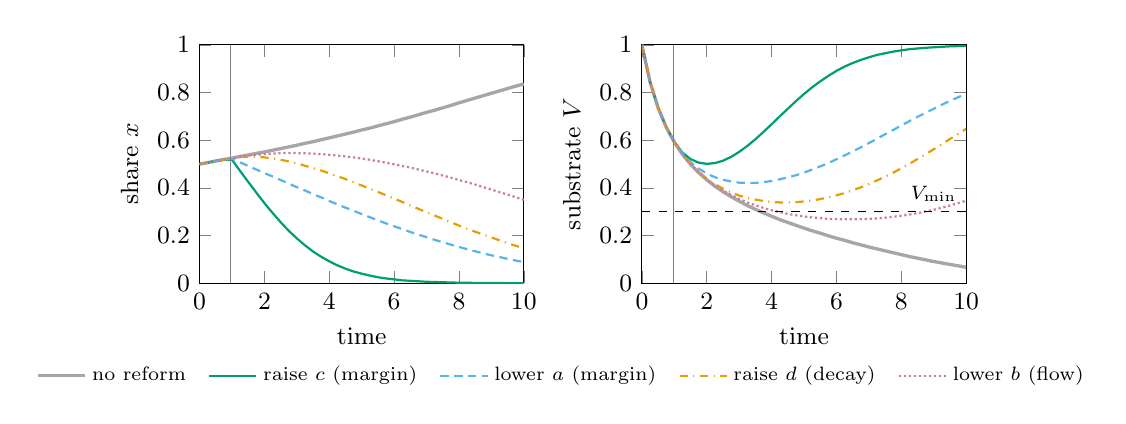
\begin{tikzpicture}
\begin{groupplot}[group style={group size=2 by 1, horizontal sep=1.5cm}, width=0.47\linewidth, height=0.38\linewidth,
  xmin=0, xmax=10, xlabel={time}, tick label style={font=\small}, label style={font=\small},
  legend cell align=left, legend columns=5, legend style={font=\scriptsize, at={(1.12,-0.3)}, anchor=north, draw=none, /tikz/every even column/.append style={column sep=6pt}}]
\nextgroupplot[ylabel={share $x$}, ymin=0, ymax=1.0]
\addplot[gray!70, very thick] coordinates {(0.000,0.500) (0.250,0.506) (0.500,0.513) (0.750,0.519) (1.000,0.525) (1.250,0.532) (1.500,0.538) (1.750,0.545) (2.000,0.551) (2.250,0.558) (2.500,0.565) (2.750,0.572) (3.000,0.579) (3.250,0.587) (3.500,0.594) (3.750,0.602) (4.000,0.610) (4.250,0.618) (4.500,0.626) (4.750,0.634) (5.000,0.643) (5.250,0.651) (5.500,0.660) (5.750,0.669) (6.000,0.678) (6.250,0.688) (6.500,0.697) (6.750,0.707) (7.000,0.717) (7.250,0.726) (7.500,0.736) (7.750,0.746) (8.000,0.757) (8.250,0.767) (8.500,0.777) (8.750,0.787) (9.000,0.797) (9.250,0.807) (9.500,0.817) (9.750,0.827) (10.000,0.836)};
\addlegendentry{no reform}
\addplot[cC, solid, thick] coordinates {(0.000,0.500) (0.250,0.506) (0.500,0.513) (0.750,0.519) (1.000,0.518) (1.250,0.471) (1.500,0.425) (1.750,0.380) (2.000,0.336) (2.250,0.295) (2.500,0.256) (2.750,0.220) (3.000,0.188) (3.250,0.159) (3.500,0.133) (3.750,0.111) (4.000,0.092) (4.250,0.075) (4.500,0.061) (4.750,0.049) (5.000,0.040) (5.250,0.032) (5.500,0.025) (5.750,0.020) (6.000,0.016) (6.250,0.012) (6.500,0.010) (6.750,0.008) (7.000,0.006) (7.250,0.005) (7.500,0.004) (7.750,0.003) (8.000,0.002) (8.250,0.002) (8.500,0.001) (8.750,0.001) (9.000,0.001) (9.250,0.001) (9.500,0.000) (9.750,0.000) (10.000,0.000)};
\addlegendentry{raise $c$ (margin)}
\addplot[cA, densely dashed, thick] coordinates {(0.000,0.500) (0.250,0.506) (0.500,0.513) (0.750,0.519) (1.000,0.522) (1.250,0.507) (1.500,0.492) (1.750,0.477) (2.000,0.462) (2.250,0.448) (2.500,0.433) (2.750,0.418) (3.000,0.403) (3.250,0.389) (3.500,0.374) (3.750,0.360) (4.000,0.345) (4.250,0.331) (4.500,0.317) (4.750,0.304) (5.000,0.290) (5.250,0.277) (5.500,0.264) (5.750,0.251) (6.000,0.239) (6.250,0.227) (6.500,0.215) (6.750,0.204) (7.000,0.193) (7.250,0.182) (7.500,0.172) (7.750,0.162) (8.000,0.152) (8.250,0.143) (8.500,0.134) (8.750,0.125) (9.000,0.117) (9.250,0.110) (9.500,0.102) (9.750,0.095) (10.000,0.089)};
\addlegendentry{lower $a$ (margin)}
\addplot[cD, dashdotted, thick] coordinates {(0.000,0.500) (0.250,0.506) (0.500,0.513) (0.750,0.519) (1.000,0.525) (1.250,0.530) (1.500,0.531) (1.750,0.531) (2.000,0.528) (2.250,0.524) (2.500,0.518) (2.750,0.511) (3.000,0.503) (3.250,0.493) (3.500,0.483) (3.750,0.473) (4.000,0.461) (4.250,0.449) (4.500,0.437) (4.750,0.424) (5.000,0.410) (5.250,0.397) (5.500,0.383) (5.750,0.369) (6.000,0.355) (6.250,0.341) (6.500,0.326) (6.750,0.312) (7.000,0.298) (7.250,0.284) (7.500,0.270) (7.750,0.256) (8.000,0.242) (8.250,0.229) (8.500,0.216) (8.750,0.204) (9.000,0.192) (9.250,0.180) (9.500,0.168) (9.750,0.157) (10.000,0.147)};
\addlegendentry{raise $d$ (decay)}
\addplot[cB, densely dotted, thick] coordinates {(0.000,0.500) (0.250,0.506) (0.500,0.513) (0.750,0.519) (1.000,0.525) (1.250,0.531) (1.500,0.536) (1.750,0.539) (2.000,0.542) (2.250,0.544) (2.500,0.546) (2.750,0.546) (3.000,0.546) (3.250,0.545) (3.500,0.544) (3.750,0.542) (4.000,0.539) (4.250,0.536) (4.500,0.532) (4.750,0.528) (5.000,0.523) (5.250,0.518) (5.500,0.512) (5.750,0.506) (6.000,0.499) (6.250,0.492) (6.500,0.485) (6.750,0.477) (7.000,0.469) (7.250,0.461) (7.500,0.452) (7.750,0.443) (8.000,0.433) (8.250,0.424) (8.500,0.414) (8.750,0.403) (9.000,0.393) (9.250,0.382) (9.500,0.372) (9.750,0.361) (10.000,0.350)};
\addlegendentry{lower $b$ (flow)}

\draw[black!50, thin] (axis cs:0.965,0) -- (axis cs:0.965,1.0);
\nextgroupplot[ylabel={substrate $V$}, ymin=0, ymax=1.0]
\addplot[gray!70, very thick] coordinates {(0.000,1.000) (0.250,0.845) (0.500,0.736) (0.750,0.655) (1.000,0.592) (1.250,0.541) (1.500,0.499) (1.750,0.464) (2.000,0.434) (2.250,0.407) (2.500,0.384) (2.750,0.363) (3.000,0.344) (3.250,0.326) (3.500,0.310) (3.750,0.295) (4.000,0.281) (4.250,0.267) (4.500,0.255) (4.750,0.243) (5.000,0.231) (5.250,0.220) (5.500,0.210) (5.750,0.199) (6.000,0.189) (6.250,0.180) (6.500,0.170) (6.750,0.161) (7.000,0.152) (7.250,0.144) (7.500,0.136) (7.750,0.128) (8.000,0.120) (8.250,0.112) (8.500,0.105) (8.750,0.098) (9.000,0.091) (9.250,0.085) (9.500,0.079) (9.750,0.073) (10.000,0.067)};
\addplot[cC, solid, thick] coordinates {(0.000,1.000) (0.250,0.845) (0.500,0.736) (0.750,0.655) (1.000,0.592) (1.250,0.548) (1.500,0.521) (1.750,0.506) (2.000,0.501) (2.250,0.504) (2.500,0.514) (2.750,0.530) (3.000,0.551) (3.250,0.576) (3.500,0.604) (3.750,0.635) (4.000,0.667) (4.250,0.700) (4.500,0.732) (4.750,0.764) (5.000,0.794) (5.250,0.822) (5.500,0.847) (5.750,0.870) (6.000,0.891) (6.250,0.909) (6.500,0.924) (6.750,0.937) (7.000,0.948) (7.250,0.958) (7.500,0.965) (7.750,0.972) (8.000,0.977) (8.250,0.982) (8.500,0.985) (8.750,0.988) (9.000,0.990) (9.250,0.992) (9.500,0.994) (9.750,0.995) (10.000,0.996)};
\addplot[cA, densely dashed, thick] coordinates {(0.000,1.000) (0.250,0.845) (0.500,0.736) (0.750,0.655) (1.000,0.592) (1.250,0.544) (1.500,0.508) (1.750,0.481) (2.000,0.460) (2.250,0.445) (2.500,0.434) (2.750,0.427) (3.000,0.422) (3.250,0.421) (3.500,0.421) (3.750,0.424) (4.000,0.429) (4.250,0.436) (4.500,0.444) (4.750,0.453) (5.000,0.464) (5.250,0.477) (5.500,0.490) (5.750,0.504) (6.000,0.520) (6.250,0.536) (6.500,0.553) (6.750,0.570) (7.000,0.588) (7.250,0.606) (7.500,0.625) (7.750,0.643) (8.000,0.662) (8.250,0.680) (8.500,0.698) (8.750,0.715) (9.000,0.732) (9.250,0.749) (9.500,0.765) (9.750,0.780) (10.000,0.795)};
\addplot[cD, dashdotted, thick] coordinates {(0.000,1.000) (0.250,0.845) (0.500,0.736) (0.750,0.655) (1.000,0.592) (1.250,0.541) (1.500,0.500) (1.750,0.467) (2.000,0.439) (2.250,0.416) (2.500,0.397) (2.750,0.381) (3.000,0.368) (3.250,0.358) (3.500,0.351) (3.750,0.345) (4.000,0.341) (4.250,0.339) (4.500,0.339) (4.750,0.340) (5.000,0.343) (5.250,0.347) (5.500,0.353) (5.750,0.360) (6.000,0.369) (6.250,0.378) (6.500,0.390) (6.750,0.402) (7.000,0.416) (7.250,0.431) (7.500,0.447) (7.750,0.464) (8.000,0.482) (8.250,0.501) (8.500,0.521) (8.750,0.541) (9.000,0.562) (9.250,0.583) (9.500,0.605) (9.750,0.626) (10.000,0.648)};
\addplot[cB, densely dotted, thick] coordinates {(0.000,1.000) (0.250,0.845) (0.500,0.736) (0.750,0.655) (1.000,0.592) (1.250,0.541) (1.500,0.500) (1.750,0.465) (2.000,0.436) (2.250,0.410) (2.500,0.389) (2.750,0.370) (3.000,0.354) (3.250,0.339) (3.500,0.327) (3.750,0.316) (4.000,0.306) (4.250,0.298) (4.500,0.291) (4.750,0.285) (5.000,0.280) (5.250,0.276) (5.500,0.273) (5.750,0.270) (6.000,0.269) (6.250,0.268) (6.500,0.268) (6.750,0.269) (7.000,0.270) (7.250,0.272) (7.500,0.275) (7.750,0.279) (8.000,0.283) (8.250,0.288) (8.500,0.294) (8.750,0.301) (9.000,0.308) (9.250,0.317) (9.500,0.326) (9.750,0.336) (10.000,0.346)};
\addplot[black, dashed, domain=0:10, samples=2] {0.3}; \node[font=\scriptsize, anchor=south east] at (axis cs:10,0.3) {$V_{\min}$};
\draw[black!50, thin] (axis cs:0.965,0) -- (axis cs:0.965,1.0);
\end{groupplot}
\end{tikzpicture}
\caption{Same destination, different paths. Running example with $h=1.5$, so harm exceeds regrowth under full capture, starting from $(x,r,V)=(0.5,0.5,1)$. At the vertical line ($V=0.6$) a reform takes $\Rcap$ from $2.5$ to $0.8$ by one of four levers: $c\to1.25$, $a\to0.32$, $d\to3.125$ or $b\to0.32$. All four end at $(0,0,K)$. The lowest substrate levels are $0.50$, $0.42$, $0.34$ and $0.27$ respectively; only the flow lever crosses $\Vmin=0.3$ (dashed). Without reform (grey), $V\to0$.}
\label{fig:levers}
\end{figure}

\section{Epistemic lag: compressible and incompressible evidence}\label{sec:lag}

\subsection{Challenge and assurance}

For a hazard class $k$, let $C_k(t)>0$ be a normalized \emph{challenge index}: the scope of behaviors, autonomy, access and diffusion that an assurance process must cover. Let $A_k(t)>0$, in the same units, be the largest challenge for which independent evidence and intervention are adequate. Write $q_k=C_k/A_k$, and call the situation acceptable when $q_k\le\qmax$. These are conceptual indices defined class by class. They do not presuppose that capability or safety is a single measurable quantity, and a scalar ``safety index'' across hazard classes would conceal the failures it is meant to reveal. Where no ambiguity arises, the index $k$ is dropped.

\paragraph{Compressible evidence.} For some classes, evidence can be produced before exposure: by testing, red-teaming, simulation or formal analysis. Assurance then grows with investment, and AI assistance can itself accelerate it \citep{perez2022}, subject to the independence conditions of Section~\ref{sec:observability}. In a stylized local approximation $C=C_0e^{\gamma t}$ and $A=A_0e^{\alpha t}$. If $\gamma>\alpha$ and $C_0/A_0<\qmax$, the ratio crosses its limit at
\begin{equation}\label{eq:crossing}
t^\ast=\frac{\ln(\qmax A_0/C_0)}{\gamma-\alpha},
\end{equation}
even though assurance improves in absolute terms. The crossing time is linear in $1/(\gamma-\alpha)$ and only logarithmic in the initial headroom. For compressible classes, $\alpha$ is a policy variable.

\subsection{Incompressible evidence and a speed limit}

Some consequences can be observed only by exposing the world to a system at the relevant level and waiting. There are four sources of such incompressibility.
\begin{itemize}[leftmargin=*]
\item \emph{Manifestation.} Some consequences are integrals over exposure. Dependency, the atrophy of skills, adjustment in labor and institutions, and shifts in belief and trust accumulate on the clocks of the systems they affect.
\item \emph{Reflexivity.} Deployment changes the environment that generates consequences. An evaluation made before deployment therefore samples a world that deployment will alter, as performative prediction \citep{perdomo2020} and the Lucas critique \citep{lucas1976} describe.
\item \emph{Irreducibility.} For coupled socio-technical systems there may be no procedure faster than the system itself for computing some consequences \citep{moore1990}. Coarse-grained regularities can nonetheless remain predictable \citep{israeli2004}, which is why the classification is made class by class.
\item \emph{Novelty.} The consequence knowledge embodied in prior experience is thickest where situations are familiar and thinnest at the frontier. Where qualitatively new behavior appears at new capability levels, extrapolation from lower levels has limited reach \citep{wei2022}, although how abruptly such behavior appears depends on how it is measured \citep{schaeffer2023}.
\end{itemize}

\begin{assumption}[Incompressible class]\label{ass:incompressible}
For hazard class $k$ there are a \emph{manifestation window} $m_k>0$ and an \emph{extrapolation reach} $\lambda_k\ge1$ such that $A_k(t)\le\lambda_k\,C_k(t-m_k)$. Adequate evidence at time $t$ covers at most $\lambda_k$ times the challenge level to which the world had been exposed $m_k$ earlier.
\end{assumption}

\begin{definition}[Epistemic lag]\label{def:lag}
The \emph{epistemic lag} of class $k$ is the delay between a change in the challenge and the arrival of evidence adequate to it. Its compressible part responds to investment in assurance; its incompressible part, $m_k$, does not.
\end{definition}

\begin{proposition}[A speed limit]\label{prop:speedlimit}
Under Assumption~\ref{ass:incompressible}, $q_k(t)\ge C_k(t)/\big(\lambda_kC_k(t-m_k)\big)$ for all $t\ge m_k$.
\begin{enumerate}[label=(\roman*),leftmargin=*]
\item If $C_k(t)=C_0e^{\gamma t}$, then $q_k\ge e^{\gamma m_k}/\lambda_k$, and acceptability for all $t$ requires
\begin{equation}\label{eq:speedlimit}
\gamma\ \le\ \frac{\ln(\lambda_k\qmax)}{m_k},
\end{equation}
whatever resources are devoted to assurance.
\item In general, acceptability requires $C_k(t)/C_k(t-m_k)\le\lambda_k\qmax$ for all $t$: the challenge may grow by at most the factor $\lambda_k\qmax$ per manifestation window.
\item The bound is attained by \emph{paced advancement}. Raise the challenge by the factor $\lambda_k\qmax$, then hold it for $m_k$ while the consequences of the new level are observed independently, and repeat.
\end{enumerate}
\end{proposition}

For compressible classes $\lambda_k$ is large, the bound~\eqref{eq:speedlimit} is slack, and the crossing time~\eqref{eq:crossing} governs. The claim that capability outruns correction is therefore not a general claim about AI. It holds for hazard classes with a small extrapolation reach and a long manifestation window, and finding those classes is an empirical program. Paced advancement is a precise form of what may be called development within understanding: the challenge advances no faster than evidence about it can form.

A uniform acceleration of every rate in a system only rescales time. The danger lies in a mismatch between clocks that accelerate and clocks that do not. Manifestation windows and the time institutions need to decide do not shrink with the pace of the technology. Irreversibility horizons, by contrast, may shrink as diffusion and integration speed up.

\subsection{The correction window}

\begin{proposition}[The correction window]\label{prop:window}
For class $k$, let $T_k$ be the irreversibility horizon, measured from the onset of exposure at a given level. Let $\tau_d$ be the time needed to decide on correction, and $\tau_r$ the time needed to reverse the exposure, which by Proposition~\ref{prop:levers} depends on the instrument.
\begin{enumerate}[label=(\roman*),leftmargin=*]
\item Correction after exposure is possible only if
\begin{equation}\label{eq:window}
m_k+\tau_d+\tau_r<T_k .
\end{equation}
\item If these durations are random, the probability of timely correction is at most $\Pr(m_k+\tau_d+\tau_r<T_k)$.
\item If $m_k\ge T_k$, no policy of exposure followed by correction is safe for class $k$. Only ex ante limits on exposure can be, or measures that lengthen $T_k$: containment, bounded reach and engineered reversibility.
\end{enumerate}
\end{proposition}

Where evaluation precedes exposure, the condition applies to the residual hazards that evaluation misses. A release schedule shorter than the evaluation it requires substitutes the absence of observed failures for evidence of their absence. Propositions~\ref{prop:speedlimit} and~\ref{prop:window} sort hazard classes into three kinds:
\begin{itemize}[leftmargin=*]
\item \emph{compressible} classes, which can be gated on a safety case made before exposure;
\item \emph{incompressible but correctable} classes, which satisfy~\eqref{eq:window} and call for paced, bounded exposure under independent observation;
\item \emph{uncorrectable} classes, with $m_k\ge T_k$ even under bounded exposure, for which exposure is excluded until the class becomes compressible or $T_k$ is lengthened.
\end{itemize}

\section{Observability and the capture of evidence}\label{sec:observability}

\subsection{What observations cannot decide}

\begin{lemma}[Indistinguishability]\label{lem:indist}
Let $\omega_1,\omega_2$ be states with safe action sets $\mathcal{S}_1,\mathcal{S}_2$ and $\mathcal{S}_1\cap \mathcal{S}_2=\emptyset$.
\begin{enumerate}[label=(\roman*),leftmargin=*]
\item If the observation is the same in both states, no decision rule, deterministic or randomized, is safe with certainty in both.
\item If the observations have distributions $P_1,P_2$, every randomized rule $\delta$ satisfies
\[
\max_{i=1,2}\Pr\nolimits_{P_i}\big(\delta\notin \mathcal{S}_i\big)\ \ge\ \tfrac12\big(1-\TV(P_1,P_2)\big).
\]
\end{enumerate}
\end{lemma}

Stronger optimization on the same observations does not escape the lemma. Only three things do: independent observation, which separates $P_1$ from $P_2$; reversible probing, which creates such separation; or an action that is safe in both states. Before a transition, declining it is typically such a common safe action. After exposure, dependency accumulates: withdrawal imposes costs on those who have come to rely on the system, and in some states withdrawal itself stops being safe. Capture thus shrinks the set of common safe actions, and this is the formal reason to decide before dependency forms.

\subsection{Capture of the evidence channel}

For incompressible classes, evidence arrives through deployment. There the deployer controls much of the measurement: access to data, the definition and reporting of incidents, the design of post-deployment monitoring, and the benchmarks used to compare systems. The measurement structure then depends on $r$, and quantitative indicators used for decisions become subject to the pressures they are meant to monitor \citep{campbell1979}. Model the observation of the substrate as $y=\varphi(V,r)$. Here $\varphi$ is continuous and strictly increasing in $V$, and $\varphi(V,0)=V$. Call capture \emph{flattering} if $\varphi(V,r)$ is nondecreasing in $r$: captured conventions report the substrate as healthier than it is. The alarm rule ``correct when $y\le\Valarm$'' is calibrated at $r=0$.

\begin{proposition}[Capture lowers the effective alarm]\label{prop:mask}
Under flattering capture, the alarm fires only when $V\le\Veff(r)$, where $\Veff(r)$ is the value of $V$ at which $\varphi(V,r)=\Valarm$ (with $\Veff(r)=0$ if $\varphi(0,r)\ge\Valarm$). $\Veff(r)\le\Valarm$, and $\Veff$ is nonincreasing in $r$. In the affine case $\varphi(V,r)=V+\beta(r)(K-V)$, with $\beta$ nondecreasing, $\beta(0)=0$ and $\beta<1$,
\[
\Veff(r)=\frac{\Valarm-\beta(r)K}{1-\beta(r)},
\]
and the alarm is silenced whenever $\beta(r)\ge\Valarm/K$. With additive observation noise of fixed distribution, the separation between two substrate levels shrinks by the factor $1-\beta(r)$, and Lemma~\ref{lem:indist}(ii) bounds the probability of an unsafe decision away from zero.
\end{proposition}

\begin{proposition}[Capture consumes the correction budget]\label{prop:budget}
In model~\eqref{eq:core}--\eqref{eq:substrate} with flattering capture and the levers of Proposition~\ref{prop:levers}, every term of the correction condition moves against correction as capture advances:
\begin{enumerate}[label=(\alph*),leftmargin=*]
\item the effective alarm level $\Veff(r)$ is nonincreasing in $r$, so detection comes later;
\item the lower bound $\ln(ar/c)/(\varepsilon d_{\mathrm{eff}})$ on the reversal latency of memory levers is increasing in $r$, so reversal takes longer;
\item the substrate's per-capita rate of decline, $hx-\rho(1-V/K)$, is increasing in $x$, so the horizon to the floor shortens.
\end{enumerate}
\end{proposition}

Figure~\ref{fig:chain} shows the budget in the running example. Without reform, $V$ falls from the alarm level $0.6$ to the floor $0.3$ in $2.7$ time units.
\begin{itemize}[leftmargin=*]
\item \emph{Delay.} The margin levers tolerate observation-plus-decision delays of at least $2.0$ and $1.8$ time units, the decay lever tolerates $0.6$, and the flow lever none.
\item \emph{Masking.} The masking produced by captured measurement acts as delay. It postpones the alarm from $t=0.97$ with no masking to $1.50$ at $\mu=0.4$ and $2.60$ at $\mu=0.7$.
\end{itemize}
The paper's chain is thus a property of one model, not five separate ones. Success raises rule support. Rule support shapes measurement. Captured measurement delays the alarm. The delay, set against a lever's own reversal time, decides whether the floor holds.

\begin{figure}[t]
\centering
% --- figure generated by figures.py (fig-chain.tex) ---
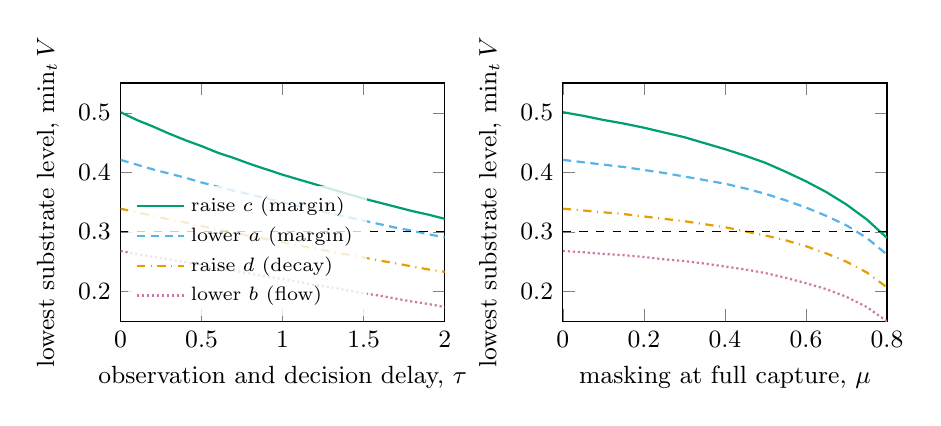
\begin{tikzpicture}
\begin{groupplot}[group style={group size=2 by 1, horizontal sep=1.5cm}, width=0.47\linewidth, height=0.38\linewidth,
  ymin=0.15, ymax=0.55, ylabel={lowest substrate level, $\min_t V$}, tick label style={font=\small}, label style={font=\small},
  legend cell align=left, legend style={font=\scriptsize, at={(0.02,0.02)}, anchor=south west, draw=none, fill=white, fill opacity=0.8, text opacity=1}]
\nextgroupplot[xlabel={observation and decision delay, $\tau$}, xmin=0, xmax=2.0]
\addplot[cC, solid, thick] coordinates {(0.000,0.501) (0.100,0.488) (0.200,0.477) (0.300,0.465) (0.400,0.454) (0.500,0.444) (0.600,0.433) (0.700,0.424) (0.800,0.414) (0.900,0.405) (1.000,0.396) (1.100,0.388) (1.200,0.380) (1.300,0.372) (1.400,0.364) (1.500,0.356) (1.600,0.349) (1.700,0.342) (1.800,0.335) (1.900,0.329) (2.000,0.322)};
\addlegendentry{raise $c$ (margin)}
\addplot[cA, densely dashed, thick] coordinates {(0.000,0.421) (0.100,0.413) (0.200,0.405) (0.300,0.398) (0.400,0.391) (0.500,0.383) (0.600,0.376) (0.700,0.369) (0.800,0.363) (0.900,0.356) (1.000,0.350) (1.100,0.343) (1.200,0.337) (1.300,0.331) (1.400,0.325) (1.500,0.319) (1.600,0.313) (1.700,0.307) (1.800,0.302) (1.900,0.296) (2.000,0.291)};
\addlegendentry{lower $a$ (margin)}
\addplot[cD, dashdotted, thick] coordinates {(0.000,0.339) (0.100,0.333) (0.200,0.327) (0.300,0.321) (0.400,0.316) (0.500,0.310) (0.600,0.304) (0.700,0.299) (0.800,0.293) (0.900,0.288) (1.000,0.283) (1.100,0.277) (1.200,0.272) (1.300,0.267) (1.400,0.262) (1.500,0.257) (1.600,0.252) (1.700,0.247) (1.800,0.242) (1.900,0.237) (2.000,0.233)};
\addlegendentry{raise $d$ (decay)}
\addplot[cB, densely dotted, thick] coordinates {(0.000,0.268) (0.100,0.263) (0.200,0.258) (0.300,0.254) (0.400,0.249) (0.500,0.244) (0.600,0.239) (0.700,0.235) (0.800,0.230) (0.900,0.225) (1.000,0.221) (1.100,0.216) (1.200,0.211) (1.300,0.207) (1.400,0.202) (1.500,0.197) (1.600,0.193) (1.700,0.188) (1.800,0.183) (1.900,0.179) (2.000,0.174)};
\addlegendentry{lower $b$ (flow)}
\addplot[black, dashed, domain=0:2.0, samples=2] {0.3};
\nextgroupplot[xlabel={masking at full capture, $\mu$}, xmin=0, xmax=0.8]
\addplot[cC, solid, thick] coordinates {(0.000,0.501) (0.050,0.495) (0.100,0.488) (0.150,0.482) (0.200,0.475) (0.250,0.467) (0.300,0.459) (0.350,0.449) (0.400,0.439) (0.450,0.428) (0.500,0.416) (0.550,0.401) (0.600,0.385) (0.650,0.367) (0.700,0.346) (0.750,0.321) (0.800,0.290)};
\addplot[cA, densely dashed, thick] coordinates {(0.000,0.421) (0.050,0.417) (0.100,0.413) (0.150,0.409) (0.200,0.404) (0.250,0.399) (0.300,0.393) (0.350,0.387) (0.400,0.381) (0.450,0.373) (0.500,0.364) (0.550,0.353) (0.600,0.341) (0.650,0.327) (0.700,0.311) (0.750,0.290) (0.800,0.262)};
\addplot[cD, dashdotted, thick] coordinates {(0.000,0.339) (0.050,0.336) (0.100,0.333) (0.150,0.330) (0.200,0.326) (0.250,0.322) (0.300,0.318) (0.350,0.313) (0.400,0.308) (0.450,0.301) (0.500,0.294) (0.550,0.286) (0.600,0.276) (0.650,0.264) (0.700,0.250) (0.750,0.232) (0.800,0.207)};
\addplot[cB, densely dotted, thick] coordinates {(0.000,0.268) (0.050,0.266) (0.100,0.263) (0.150,0.261) (0.200,0.258) (0.250,0.254) (0.300,0.251) (0.350,0.247) (0.400,0.242) (0.450,0.237) (0.500,0.231) (0.550,0.223) (0.600,0.214) (0.650,0.204) (0.700,0.191) (0.750,0.174) (0.800,0.150)};
\addplot[black, dashed, domain=0:0.8, samples=2] {0.3};
\end{groupplot}
\end{tikzpicture}
\caption{The correction budget in the running example. A reform fires when the observed substrate reaches $0.6$; the floor is $0.3$ (dashed). (a) Lowest substrate level against the delay between the alarm and the reform, for the four levers of Figure~\ref{fig:levers}. (b) The same against masking by captured measurement, $\beta(r)=\mu\min\{1,rd/b\}$, with no delay. Masking acts as delay.}
\label{fig:chain}
\end{figure}

\subsection{Cross-domain reinforcement}

The feedback need not stay within one market. A developer's commercial success can fund evaluation infrastructure; evaluation standards shape procurement; procurement funds the next generation of development. Let $z\ge0$ record small deviations in the activity of such channels. Near a low-capture configuration, linearize as $\dot z=(G-D)z$, where $G\ge0$ is the matrix of cross-channel reinforcement and $D$ is a positive diagonal matrix of decay rates.

\begin{lemma}[Joint threshold]\label{lem:mmatrix}
The origin is locally stable if $\spr(D^{-1}G)<1$, and has a growing direction if $\spr(D^{-1}G)>1$. Irreducibility is not required. Reducing any entry of $G$ weakly lowers $\spr(D^{-1}G)$.
\end{lemma}

For two channels with unit decay and mutual coupling $\theta$, the eigenvalues of $G-D$ are $-1\pm\theta$. Each channel decays on its own, yet the pair grows when $\theta>1$. This is the next-generation threshold familiar from epidemiology \citep{vandendriessche2002}. It shows how channels that are each subcritical can be jointly supercritical, and why firewalls between channels, which reduce the off-diagonal entries of $G$, are a lever in their own right.

\section{Coordination, founding restraint and the anatomy of a pause}\label{sec:pause}

\subsection{The race as a coordination problem}

When a practice has a private advantage and externalized costs ($c\le0$), the situation is a social dilemma: the practice dominates, and only changed payoffs, through the margin levers, change the outcome. Recursive capture turns the case $c>0$ into something different. Remark~\ref{rem:riskdominance} showed that rule memory creates positive frequency dependence, so both conventions are equilibria. Suppose the substrate cost under full capture exceeds the advantage the rules generate, $\Pi_0(K)-\Pi_0(V_H)>ab/d-c$, where $V_H$ is the substrate level under full capture. Then the no-capture convention is better for everyone, and the game is a stag hunt whose inferior equilibrium is held in place by accumulated rules \citep{skyrms2004}. The obstacle is then assurance and the state of the rules, not only incentives.

\subsection{Founding restraint and its window}

\begin{proposition}[The restraint window]\label{prop:restraint}
Let $\Rcap>1$. A coalition holding share $s$ that abandons the practice moves the state from $(x_0,r_0)$ to $(x_0-s,r_0)$. Capture then unwinds without any agreement if $x_0-s<\sigma(r_0)$, and persists if $x_0-s>\sigma(r_0)$. The minimal coalition,
\[
s^\ast(x_0,r_0)=\max\{0,\;x_0-\sigma(r_0)\},
\]
is nondecreasing in inherited rule support $r_0$ and tends to $x_0$ as $r_0\to\infty$. If the coalition also withdraws rule support $\theta s$, the condition becomes $x_0-s<\sigma(r_0-\theta s)$, which is weaker.
\end{proposition}

This reconciles two claims that appear to conflict. An appeal for one small actor to slow down while others continue is weak, because its share is far below $s^\ast$. Restraint by actors whose share is comparable to $s^\ast$ is not weak: it moves the state across the separatrix without any agreement. The window for such founding acts narrows as rule support accumulates.

Costly restraint also works through beliefs. In assurance games, costly unilateral steps by actors who would gain from proceeding are credible signals of type \citep{kydd2000}. The 1974 call by leading researchers to defer certain recombinant-DNA experiments preceded the Asilomar conference and the oversight regime that followed \citep{berg1974,berg1975}. Restraint without verification remains scaffolding. The moratorium on nuclear testing observed from 1958 ended with the resumption of Soviet testing in 1961, after negotiations over inspection had stalled \citep{divine1978}. The treaty that followed in 1963 banned only the tests that could be detected without inspection, and left underground testing, whose verification required it, outside the ban \citep{seaborg1981}.

\subsection{What a pause does}

\begin{proposition}[A pause resets rule support]\label{prop:pause}
Let $\Rcap>1$. Suppose covered transitions are paused for a duration $\Delta$. The share is frozen at $x_p\in(0,1)$, while rule support follows $\dot r=\varepsilon(b_px_p-dr)$, where $b_p$ is the rate at which shares convert into rules during the pause. Then $r\to b_px_p/d$, and after release with the original parameters, for $\Delta$ sufficiently long:
\begin{enumerate}[label=(\roman*),leftmargin=*]
\item with ordinary rule-making ($b_p=b$), the state converges to $L$ if $x_p<1/\Rcap$ and to $H$ if $x_p>1/\Rcap$;
\item with rule-making insulated from market shares ($b_p=0$), the state converges to $L$ whenever $x_p<\sigma(0)$, and $\sigma(0)>1/\Rcap$.
\end{enumerate}
\end{proposition}

A long pause under ordinary rule-making therefore unwinds capture carried by inherited rules. It also completes capture by a practice that already holds more than the saddle share, because the pause gives the rules time to catch up with the frozen shares. The warning that a pause can entrench incumbents is thus a theorem of the model, and the model also names the remedy: insulate rule-making while the pause lasts.

\begin{corollary}[Restraint and pause together]\label{cor:together}
From $(x_0,r_0)$, a coalition of share $s$ unwinds capture in three cases:
\begin{itemize}[leftmargin=*]
\item by restraint alone, if $x_0-s<\sigma(r_0)$;
\item followed by a long pause under ordinary rule-making, if $x_0-s<1/\Rcap$;
\item followed by a long pause under insulated rule-making, if $x_0-s<\sigma(0)$.
\end{itemize}
While inherited rule support is below its saddle value ($r_0<c/a$), an ordinary pause requires a larger coalition than no pause at all.
\end{corollary}

In the running example, starting from $x_0=0.95$ with $r_0=1$, the required coalition is $0.86$ for restraint alone, $0.55$ with an ordinary pause, and $0.27$ with an insulated pause (Figure~\ref{fig:coalition}).

\begin{figure}[t]
\centering
% --- figure generated by figures.py (fig-coalition.tex) ---
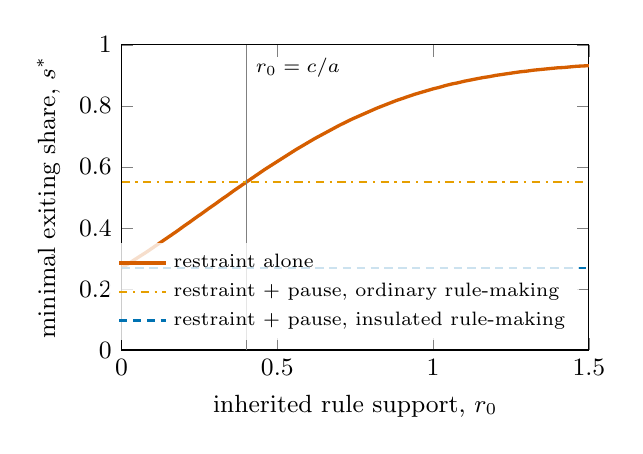
\begin{tikzpicture}
\begin{axis}[width=0.62\linewidth, height=0.45\linewidth, xmin=0, xmax=1.5, ymin=0, ymax=1,
  xlabel={inherited rule support, $r_0$}, ylabel={minimal exiting share, $s^\ast$}, tick label style={font=\small},
  label style={font=\small}, legend cell align=left, legend style={font=\scriptsize, at={(0.98,0.03)}, anchor=south east, draw=none, fill=white, fill opacity=0.8, text opacity=1}]
\addplot[cH, very thick] coordinates {(0.000,0.269) (0.020,0.281) (0.040,0.295) (0.060,0.308) (0.080,0.321) (0.100,0.335) (0.120,0.349) (0.140,0.363) (0.160,0.377) (0.180,0.391) (0.200,0.406) (0.220,0.420) (0.240,0.435) (0.260,0.449) (0.280,0.464) (0.300,0.478) (0.320,0.493) (0.340,0.507) (0.360,0.522) (0.380,0.536) (0.400,0.550) (0.420,0.564) (0.440,0.578) (0.460,0.592) (0.480,0.605) (0.500,0.618) (0.520,0.631) (0.540,0.644) (0.560,0.657) (0.580,0.669) (0.600,0.681) (0.620,0.693) (0.640,0.704) (0.660,0.715) (0.680,0.726) (0.700,0.737) (0.720,0.747) (0.740,0.757) (0.760,0.766) (0.780,0.775) (0.800,0.784) (0.820,0.793) (0.840,0.801) (0.860,0.809) (0.880,0.817) (0.900,0.824) (0.920,0.831) (0.940,0.838) (0.960,0.844) (0.980,0.850) (1.000,0.856) (1.020,0.861) (1.040,0.867) (1.060,0.872) (1.080,0.876) (1.100,0.881) (1.120,0.885) (1.140,0.889) (1.160,0.893) (1.180,0.896) (1.200,0.900) (1.220,0.903) (1.240,0.906) (1.260,0.909) (1.280,0.912) (1.300,0.914) (1.320,0.917) (1.340,0.919) (1.360,0.921) (1.380,0.923) (1.400,0.925) (1.420,0.926) (1.440,0.928) (1.460,0.930) (1.480,0.931) (1.500,0.932)};
\addlegendentry{restraint alone}
\addplot[cD, thick, dashdotted, domain=0:1.5, samples=2] {0.5500};
\addlegendentry{restraint + pause, ordinary rule-making}
\addplot[cL, thick, densely dashed, domain=0:1.5, samples=2] {0.2686};
\addlegendentry{restraint + pause, insulated rule-making}
\draw[black!50, thin] (axis cs:0.4,0) -- (axis cs:0.4,1);
\node[font=\scriptsize, anchor=north west] at (axis cs:0.4,0.99) {$r_0=c/a$};
\end{axis}
\end{tikzpicture}
\caption{The restraint window in the running example ($x_0=0.95$). The curves show the minimal share $s^\ast$ that must abandon the captured practice for capture to unwind. Under restraint alone (solid), $s^\ast$ rises with inherited rule support $r_0$. It is lower with a long pause under ordinary rule-making (dash-dot), and lower still with a long pause under rule-making insulated from market shares (dashed). Left of $r_0=c/a$, an ordinary pause is worse than none.}
\label{fig:coalition}
\end{figure}

\subsection{Pauses and accumulation}

\begin{proposition}[Accumulation]\label{prop:accumulation}
Consider a compressible class. During a pause of length $\Delta$, the deployed challenge is held constant, the latent challenge (what could be deployed at its end) grows at rate $\gamma_p$, and assurance grows at rate $\alpha_p$. On resumption to the latent frontier, $q=q(0)\,e^{(\gamma_p-\alpha_p)\Delta}$. The pause improves the ratio relative to no pause if and only if $\gamma_p-\alpha_p<\gamma-\alpha$, and reduces it outright if and only if $\alpha_p>\gamma_p$.
\end{proposition}

A pause that leaves the growth of latent capability and of assurance unchanged returns the same ratio as no pause. Its value comes from governing the inputs to latent capability and redirecting effort toward assurance, the program of differential technological development \citep{bostrom2002}. For incompressible classes the logic differs. A pause on new transitions lets existing exposure at the current level be observed for the manifestation window, so it is the waiting half of paced advancement (Proposition~\ref{prop:speedlimit}), provided the observation is independent. Elapsed time helps only through what changes while it passes:
\begin{itemize}[leftmargin=*]
\item for compressible classes, assurance;
\item for incompressible classes, the elapse of manifestation windows at a fixed level;
\item under insulated rule-making, the decay of rule support.
\end{itemize}

\section{From uncertainty to a decision rule}\label{sec:decision}

Consider a step with incremental benefit $B\ge0$ relative to delay, and an irreversible loss $\Lambda>0$ that occurs with probability $p\in[p_-,p_+]$. The maxmin rule prefers delay if $p_+\Lambda>B$ \citep{gilboa1989}. This assumes that delay avoids the risk rather than postponing it or moving it to less accountable actors. When it does not, the comparison is between the worst-case probabilities with and without delay, and the costs of restraint belong in $B$.

The rule acquires force when learning is possible. If delay produces information that narrows the probability set before a decision becomes irreversible, waiting has quasi-option value \citep{arrowfisher1974,henry1974,gollier2000}. For compressible classes, a pause produces such information through testing. For incompressible classes, information requires exposure. The relevant choice is then between advancing in large steps and advancing in paced, bounded steps whose consequences are observed before the next.

The same results fix where the burden of proof lies. By Assumption~\ref{ass:incompressible}, evidence of hazard from deployed systems arrives after the manifestation window. By Proposition~\ref{prop:mask}, it passes through channels shaped by the rule support of the practice under assessment. A rule that waits for proof of hazard therefore fires late, or not at all, in the classes where firing matters most. This paper proposes a procedural rule instead. Before a transition that substantially expands both capability and exposure, the proponent provides an auditable safety case for the foreseeable hazard classes \citep{clymer2024,buhl2024}. The case must survive independent challenge and include a withdrawal path that has been exercised. The trigger for restraint is the absence of a passing independent safety case, not the presence of demonstrated hazard.

In this sense, a transition is \emph{beyond understanding} when decisions about it cannot be supported by reliable observation, calibrated tests and timely intervention. Understanding here does not require that every internal representation of a model be interpretable. The rule is not a license for any pause a pessimist can defend. It is released by a safety case that passes, and Section~\ref{sec:tests} states the observations that would weaken the case for restraint in any given class.

\section{Three paired domains}\label{sec:domains}

Capability and correction are not two civilization-wide quantities. The relation between them has to be shown domain by domain, naming in each the capability being scaled, its corrective feedback, the delays, the thresholds and the controls. Table~\ref{tab:domains} gives three sketches. They are structural readings of the model, not measurements. The data that would parametrize them are listed in Section~\ref{sec:tests}.

\begin{table}[t]
\centering
\small
\renewcommand{\arraystretch}{1.25}
\begin{tabularx}{\linewidth}{@{}>{\raggedright\arraybackslash}p{2.3cm}>{\raggedright\arraybackslash}X>{\raggedright\arraybackslash}X>{\raggedright\arraybackslash}X@{}}
\toprule
 & Biological misuse assistance & Agents with access to software and infrastructure & The information ecosystem \\
\midrule
Capability scaled & Lowering the expertise needed to acquire, produce or use dangerous agents & Length, reliability and reach of autonomous task completion & Persuasion, personalization and generation at scale; companionship and advice \\
Evidence & Partly compressible (controlled evaluations); residual evidence arrives, if at all, after an event & Compressible for specified tasks; incompressible for open-ended, long-horizon and multi-agent behavior & Incompressible and reflexive: effects on belief, trust and attention accumulate over years \\
$m_k$ against $T_k$ & $T_k$ short once a transmissible agent is released; for residual risk, $m_k\ge T_k$ & $T_k$ set by the reach of permissions; dependency erodes withdrawal & $m_k$ long; $T_k$ uncertain, since shared reference points rebuild slowly \\
Capture channel & Threat models and test design negotiated with developers; access to evaluation at developers' consent & Incident definitions, logging and disclosure controlled by deployers; evaluation built on deployers' scaffolds & Data access controlled by deployers; the substrate $V$ is itself the capacity for independent correction \\
Implied instrument & Pre-exposure gate on a passing safety case; access controls; uncorrectable residual classes excluded & Staged permissions as the unit of exposure; engineered rollback and audit; independent incident reporting; paced advancement & Paced advancement with independent data access as an exit condition; bounded exposure \\
\bottomrule
\end{tabularx}
\caption{Three hazard domains read through the model. The rows correspond to the quantities of Sections~\ref{sec:capture}--\ref{sec:observability}.}
\label{tab:domains}
\end{table}

Three features of the table matter for the argument. The domains fall into different classes of Proposition~\ref{prop:window}, so no single instrument fits all three. The capture channel is most direct in the information ecosystem, where deployers hold the data needed to observe the substrate. There, independent researcher access, of the kind created for very large online platforms by the EU Digital Services Act \citep{eudsa2022}, is the independence condition in practice. And the evidence available today is one-sided. Task-completion horizons of frontier agents have grown approximately exponentially on METR's benchmark distribution. METR stresses that its tasks are mainly well-specified software, machine-learning and cybersecurity tasks, that the measure is of difficulty rather than real-world autonomy, and that estimates become unreliable beyond the range of its task suite \citep{metr2025,metr2026}. Such series measure the challenge $C$. Nothing comparable yet measures assurance $A$ in any domain.

\section{A conditional frontier regime}\label{sec:regime}

The regime below follows from the models. Table~\ref{tab:mapping} records the correspondence.

\paragraph{Object.} The object of restraint is an \emph{exposure-creating transition}, specified operationally. Three examples: a training run that crosses a jointly agreed capability or risk trigger; a broad release of a system whose dangerous affordances are unresolved; and granting autonomous access to high-impact infrastructure, replication channels or critical decision processes. Training compute is one trigger among several. Algorithmic progress, fine-tuning, inference-time compute and scaffolding also change effective capability \citep{hooker2024}, so triggers need periodic revision and safeguards against threshold gaming.

\paragraph{Instruments by class.} Following Section~\ref{sec:lag}:
\begin{itemize}[leftmargin=*]
\item transitions whose hazards are compressible are gated on a passing independent safety case;
\item incompressible but correctable classes advance by bounded steps, each held for its manifestation window under independent observation;
\item uncorrectable classes are excluded from exposure until evidence becomes compressible or the irreversibility horizon is lengthened by containment or bounded reach.
\end{itemize}
The last category corresponds to the ``red lines'' proposed in scientists' consensus statements \citep{idais2024}.

\paragraph{Trigger and burden.} The trigger is the absence of a passing independent safety case (Section~\ref{sec:decision}). The exit test requires four things:
\begin{itemize}[leftmargin=*]
\item evidence that bounds the specified harms to an agreed standard;
\item tests shown to remain informative under distribution shift;
\item intervention demonstrably faster than the relevant irreversibility horizon;
\item monitoring and rollback that have been exercised, not only planned.
\end{itemize}
Reasons for release or continued restraint are published.

\paragraph{The regime's own $\Rcap<1$.} A pause regime is itself a selection environment and can be captured (Proposition~\ref{prop:pause}). Its design therefore applies the four levers to itself:
\begin{itemize}[leftmargin=*]
\item \emph{Flow ($b$).} Standard-setting, evaluator funding and evaluator access are insulated from the market success of those evaluated, including while a pause is in force.
\item \emph{Decay ($d$).} Criteria lapse unless re-justified, and evaluators rotate.
\item \emph{Neutrality ($a$).} Criteria are defined by reference to hazards, not to incumbents' systems.
\item \emph{Margin ($c$).} Liability attaches to harms from covered transitions, because margin levers are the fast ones (Proposition~\ref{prop:levers}).
\end{itemize}
An evaluator counts as independent only with respect to the relevant failure mode, funding, test data, access, and the power to trigger correction; an organizational label is not enough.

\paragraph{Accumulation and reallocation.} A pause that freezes deployment while inputs accumulate dams pressure, and resumption then settles as a sharper race (Proposition~\ref{prop:accumulation}). The regime therefore governs inputs to latent capability, such as the allocation of compute to the largest runs, and directs effort toward assurance, verification and monitoring during the pause.

\paragraph{Reciprocity and founding acts.} An initial agreement can begin among willing major developers and jurisdictions, with an expandable verification perimeter and explicit treatment of non-participants. Proposition~\ref{prop:restraint} gives the order of operations:
\begin{enumerate}[leftmargin=*]
\item legible restraint by the most capable actors while rule support is still small, since the window narrows as it accumulates;
\item insulation of rule-making during the pause (Corollary~\ref{cor:together});
\item verification, which converts restraint into structure \citep{shavit2023,wasil2024,baker2025}, and graduated, reversible responses to defection \citep{axelrod1984,ostrom1990}.
\end{enumerate}
Verification remains technically immature, so ``a treaty can be verified today'' would overstate it. Coordination among developers alone raises antitrust questions \citep{alaga2023}, which favors public-law vehicles over private agreements.

\paragraph{Is this licensing?} In part it is: the exit test is an approval of a covered transition. The closest institutional analogues are conditional approvals, not moratoria:
\begin{itemize}[leftmargin=*]
\item pre-market approval backed by a safety case, as for pharmaceuticals;
\item declaration and inspection, as in nuclear safeguards;
\item tiers of containment, as in biosafety;
\item grounding orders with an exit that requires demonstrated correction, as in aviation.
\end{itemize}
After the grounding of the Boeing 737 MAX, return to service in November 2020 followed required design changes rather than elapsed time \citep{faa2020}. During recertification, the regulator kept the compliance findings for those changes instead of delegating them to the manufacturer's designated organization \citep{dotoig2023}. That is a lowering of $b$, in the terms of this paper.

\paragraph{What exists and what is added.} Obligations for general-purpose models with systemic risk under the EU AI Act \citep{euaiact2024,eucop2025}, California's frontier framework and incident-reporting requirements \citep{sb53}, developers' frontier safety frameworks and the Seoul commitments already require much of the evidence above. The regime adds four things: evaluation independent of the evaluated, reciprocity, exits that differ by hazard class, and anti-capture design applied to itself.

\paragraph{Costs of restraint.} Restraint has real costs:
\begin{itemize}[leftmargin=*]
\item concentration of power;
\item lost health and scientific benefits;
\item geopolitical instability;
\item reduced defensive capability;
\item relocation of development to less accountable actors.
\end{itemize}
To these the model adds its own warning: a pause regime can be captured. These costs enter $B$ in the decision rule and constrain the design; they are not rhetorical exceptions.

\begin{table}[t]
\centering
\small
\renewcommand{\arraystretch}{1.2}
\begin{tabularx}{\linewidth}{@{}>{\raggedright\arraybackslash}p{4.2cm}>{\raggedright\arraybackslash}X>{\raggedright\arraybackslash}p{3.2cm}@{}}
\toprule
Regime element & Model quantity & Source \\
\midrule
Trigger: no passing safety case & Evidence arrives after $m_k$, through channels shaped by $r$ & Assumption~\ref{ass:incompressible}; Prop.~\ref{prop:mask} \\
Gate for compressible classes & Hold $C$ while $A$ grows; exit when $q\le\qmax$ & Eq.~\eqref{eq:crossing}; Prop.~\ref{prop:accumulation} \\
Paced advancement & Growth factor $\le\lambda_k\qmax$ per window $m_k$ & Prop.~\ref{prop:speedlimit} \\
Exclusion of uncorrectable classes & $m_k\ge T_k$ & Prop.~\ref{prop:window} \\
Exercised rollback & Measured $\tau_r$ in~\eqref{eq:window} & Props.~\ref{prop:levers},~\ref{prop:window} \\
Independent evaluation & $\varphi$ independent of $r$; $\TV$ separation & Lemma~\ref{lem:indist}; Prop.~\ref{prop:mask} \\
Insulated rule-making ($b$) & Regime's own $\Rcap<1$; insulation during pauses & Props.~\ref{prop:capture},~\ref{prop:pause} \\
Sunset and rotation ($d$) & Decay of accumulated rule support & Prop.~\ref{prop:levers} \\
Liability ($c$) & Margin lever with no latency & Prop.~\ref{prop:levers}(i) \\
Firewalls between channels & Off-diagonal entries of $G$ & Lemma~\ref{lem:mmatrix} \\
Governing inputs & Latent growth $\gamma_p$ during a pause & Prop.~\ref{prop:accumulation} \\
Early, legible restraint & Restraint window $s^\ast(r_0)$ & Prop.~\ref{prop:restraint} \\
\bottomrule
\end{tabularx}
\caption{How the elements of the regime follow from the model.}
\label{tab:mapping}
\end{table}

\section{Discriminating tests and refutation}\label{sec:tests}

Each mechanism makes predictions that can fail.
\begin{itemize}[leftmargin=*]
\item \emph{Recursive capture.} Successful deployments should shift evaluation, procurement or access rules in their own favor after confounders are controlled for. A multi-actor sandbox can separately toggle the reward for current performance and the channel from performance to future rule-setting. If the second toggle has no mediated effect on persistence, the distinctive mechanism adds little. Matched systems with different rule histories should diverge, although hidden resources and fixed switching costs must also be checked.
\item \emph{Bistability.} As a system approaches a capture threshold, recovery from perturbations should slow, with rising autocorrelation and variance in adoption shares and in rule support \citep{scheffer2009}. Abrupt transitions without such signatures count against the bistable model in that domain.
\item \emph{Lever latency.} Reforms on the margin (liability, internalized cost) should change behavior faster than reforms on the stock of rules (revised standards, sunsets), and these faster than reforms on the flow (insulated future rule-making). Regulatory histories can test the ordering.
\item \emph{Incompressibility.} For a given hazard class, pre-deployment evaluation may reliably predict deployment-stage findings, and the lag from deployment to discovery may shrink as evaluation investment grows. If so, the class is compressible and the speed limit does not bind for it.
\item \emph{Capture of evidence.} Divergence between deployer-reported and independently measured indicators should grow with the deployer's share and rule influence.
\item \emph{Restraint window.} The effect of unilateral restraint on others' behavior should depend on the restraining actors' share relative to accumulated rule support.
\end{itemize}

\paragraph{When the case for slowdown weakens.} The case for a particular slowdown weakens in any of four circumstances: independent assurance reliably keeps pace with capability and exposure in the relevant classes; severe harms are reversible before their functional threshold; competitors maintain effective scrutiny without common restraint; or delay creates larger plausible irreversible harms. It strengthens if tests repeatedly lag release, if discovered hazards fail to affect deployment, or if evaluation and remedy cannot observe the relevant states. Dismissing contrary evidence as proof that critics have been captured would itself be an epistemic failure.

\paragraph{Data.} Several data streams would make the framework usable:
\begin{itemize}[leftmargin=*]
\item the delay from release to evaluation;
\item the time from incident detection to effective mitigation;
\item capability and reach, task by task;
\item deployments made despite unresolved findings;
\item evaluator independence and access;
\item the survival of alternative providers;
\item changes in oversight that follow commercial success;
\item discovery lags by hazard class.
\end{itemize}
Confidential incident data may require trusted access rather than indiscriminate publication. None of the parameters in this paper has been calibrated with such data, and numerical thresholds for a real pause cannot be read off the equations.

\section{Limits and conclusion}\label{sec:conclusion}

The models are deliberately small. They leave out:
\begin{itemize}[leftmargin=*]
\item beneficial feedback and innovation in assurance;
\item multiple competing practices and heterogeneous actors;
\item strategic concealment and state rivalry;
\item the asymmetric feedback of the substrate onto payoffs.
\end{itemize}
The manifestation window and the extrapolation reach are primitives, and estimating them is itself an empirical program. The regime inherits the political difficulty of any international arrangement. The substrate variable exposes a logical separation; it is not a quantified prediction of civilization's viability. Nothing here shows that current frontier development has crossed an irreversible boundary, that one policy fits every jurisdiction, or that indefinite cessation is justified.

There is nonetheless a defensible reason to reject unconditional acceleration of the frontier. The capacity to build and distribute powerful systems and the capacity to understand, contest and withdraw them are different processes, running on different clocks. Some of those clocks cannot be accelerated. Success converts into the rules that measure it, and so lengthens both the detection and the reversal of error while it shortens the horizon within which error can still be corrected.

The appropriate response has three parts:
\begin{itemize}[leftmargin=*]
\item restraint targeted at transitions whose evidence cannot yet be had;
\item paced, bounded advancement where evidence requires exposure;
\item separation of success from rule-setting, including within the regime that restrains.
\end{itemize}
The position requires neither hostility to AI nor a confident prediction of disaster. It asks that the ability to change our collective course remain real while the stakes and the speed rise.

\section*{Author note on assistance and verification}
This manuscript was developed with substantive assistance from AI language models. An unnamed AI tool drafted the first version at the author's request. Claude Opus~5.5 (Anthropic) revised and extended this version after two AI reviews of the first, one by Claude Opus~5.5 and one by Claude Fable~5.1. The figures and every number quoted in the text are computed by a script distributed with the manuscript. The named author must review and take responsibility for every claim, equation, citation and policy recommendation before submission. No empirical study is claimed, and the numerical results illustrate the propositions; they are not estimates.

\appendix
\section{Proofs}\label{app:proofs}

\begin{proof}[Proof of Proposition~\ref{prop:capture}]
The lines $x=0$ and $x=1$ are invariant, and on $r=0$ we have $\dot r=\varepsilon bx\ge0$, so $[0,1]\times[0,\infty)$ is forward invariant. Since $x\le1$, $\dot r\le\varepsilon(b-dr)$, and hence
\[
r(t)\le r(0)e^{-\varepsilon dt}+(b/d)(1-e^{-\varepsilon dt})\le\max\{r(0),b/d\}.
\]

(i) If $\Rcap<1$ then $ab/d<c$. Since $\limsup_t r(t)\le b/d$, there are $T$ and $\delta>0$ with $ar(t)-c\le-\delta$ for $t\ge T$. Then $\tfrac{\dd}{\dd t}\logit x=\kappa(ar-c)\le-\kappa\delta$, so $x\to0$ whenever $x(0)\in(0,1)$, and then $\dot r=\varepsilon(bx-dr)$ gives $r\to0$. If $x(0)=0$, the solution stays on $x=0$ and $r\to0$.

(ii)--(iii) The equilibria follow from $\dot x=0$ (so $x\in\{0,1\}$ or $r=c/a$) together with $\dot r=0$ (so $r=bx/d$). The Jacobian is
\[
J=\begin{pmatrix}\kappa(1-2x)(ar-c)&\kappa ax(1-x)\\ \varepsilon b&-\varepsilon d\end{pmatrix}.
\]
Its eigenvalues are $-\kappa c$ and $-\varepsilon d$ at $L$, and $-\kappa c(\Rcap-1)$ and $-\varepsilon d$ at $H$. At $S$, $J_{11}=0$ and $\det J=-\kappa\varepsilon ab\,x_S(1-x_S)<0$, so $S$ is a saddle.

For $\Phi$, $\partial_x\Phi=ar-c$ and $\partial_r\Phi=(a/b)(bx-dr)$, which give the gradient form and
\[
\dot\Phi=\kappa x(1-x)(ar-c)^2+\tfrac{\varepsilon a}{b}(bx-dr)^2\ge0 .
\]
Here $\dot\Phi=0$ requires $bx=dr$ and $x(1-x)(ar-c)=0$, which holds only at $L$, $H$ and $S$. Solutions are bounded. By LaSalle's invariance principle \citep{lasalle1960}, every $\omega$-limit set is a connected subset of $\{L,H,S\}$, hence a single equilibrium. The stable manifold of the hyperbolic saddle $S$ is a curve, and solutions not on it converge to $L$ or $H$.

The system is cooperative ($\partial\dot x/\partial r\ge0$, $\partial\dot r/\partial x>0$) and irreducible in the interior. For such planar systems, the stable manifold of a saddle is unordered: no two of its points are ordered componentwise \citep{hirsch1985,smith1995}. It is therefore the graph of a nonincreasing function $x=\sigma(r)$, and $\sigma(c/a)=1/\Rcap$.

Consider first the branch above $S$. Since $\Phi$ increases strictly along non-constant solutions, no solution returns to $S$, and the sinks $L$ and $H$ cannot be $\alpha$-limit points. So in backward time the branch leaves every compact set, and because it cannot cross the invariant line $x=0$, it does so with $r\to\infty$. To see that $\sigma(r)\to0$, fix $x_0>0$ and let $t_1=\ln\big(ar_0/(2c)\big)/(\varepsilon d)$. Since $r(t)\ge r_0e^{-\varepsilon dt}$, on $[0,t_1]$ we have $ar-c\ge c$, so $\logit x(t_1)\ge\logit x_0+\kappa ct_1$ while $r(t_1)\ge 2c/a$. For $r_0$ large, $(x(t_1),r(t_1))\in Q_H$, so $(x_0,r_0)$ lies in the basin of $H$ and $\sigma(r_0)\le x_0$.

The branch below $S$ leaves the domain through $r=0$, where $\dot r>0$. It cannot reach the invariant line $x=1$, so $\sigma(0)<1$. And $\sigma(0)>1/\Rcap$, because on the segment $x=1/\Rcap$, $0\le r<c/a$ we have $\dot x<0$, so that segment is not invariant.

(iv) On the boundary of $Q_H$, $\dot x>0$ at $x=1/\Rcap$ with $r>c/a$, and $\dot r=\varepsilon b(x-1/\Rcap)>0$ at $r=c/a$ with $x>1/\Rcap$. So $Q_H$ is forward invariant. Inside it $x$ increases to $1$, and then $r\to b/d$. The argument for $Q_L$ is symmetric, and inside $Q_L$ we have $x\to0$ and then $r\to0$.
\end{proof}

\begin{proof}[Remarks~\ref{rem:clocks} and~\ref{rem:riskdominance}]
As $\varepsilon/\kappa\to0$, $x$ relaxes to $0$ or $1$ according to the sign of $ar-c$ before $r$ moves appreciably, so the fate is decided by whether $r(0)$ exceeds $c/a$. As $\varepsilon/\kappa\to\infty$, $r$ relaxes to $bx/d$ first, and the fate is decided by whether $x(0)$ exceeds $1/\Rcap$.

In the reduction $r=bx/d$, $\dot x=\kappa c\,x(1-x)(\Rcap x-1)$. The basin of $x=1$ is $(1/\Rcap,1]$, which is larger than that of $x=0$ exactly when $\Rcap>2$. Along the reduction, $\Phi(x,bx/d)=cx(\Rcap x/2-1)$, which is maximized at $x=1$ exactly when $\Rcap>2$. For symmetric $2\times2$ coordination games, the risk-dominant equilibrium is the potential maximizer and is the stochastically stable one \citep{kandori1993,young1993}.
\end{proof}

\begin{proof}[Proof of Proposition~\ref{prop:substrate}]
Near the hyperbolic sink $H$, convergence is exponential, so $\int_0^\infty(1-x)\,\dd t<\infty$. Write $\dot V=V[(\rho-h)+h(1-x)-\rho V/K]$.

If $h>\rho$, then $V(t)\le V(0)\exp\big((\rho-h)t+h\int_0^t(1-x)\big)\to0$ exponentially.

If $h=\rho$, then $u=1/V$ satisfies $\dot u=-\rho(1-x)u+\rho/K$. Hence $u(t)\ge e^{-M}(u(0)+\rho t/K)$ with $M=\rho\int_0^\infty(1-x)$, and so $V(t)\le e^{M}K/(\rho t)$.

If $h<\rho$, fix $\eta>0$. Eventually $hx\in(h-\eta,h]$, so $V$ lies between solutions of the logistic equations with intrinsic rates $\rho-h$ and $\rho-h+\eta$. Letting $\eta\to0$ gives $V\to K(1-h/\rho)$.

The case $(x,r)\to L$ is the same with $x\to0$.
\end{proof}

\begin{proof}[Proof of Proposition~\ref{prop:viability}]
(i) Since $hx\le h\bar x$, $V\ge W$ by comparison, where $\dot W=W[\rho(1-W/K)-h\bar x]$ and $W(0)=V(0)$. The positive equilibrium of $W$ is $K(1-h\bar x/\rho)=\Vmin$, and $W(0)\ge\Vmin$, so $W(t)\ge\Vmin$ for all $t$.

(ii) On the rectangle $[0,\bar x]\times[0,c/a)$ we have $\dot x\le0$. At $r=c/a$ with $x\le\bar x<1/\Rcap$ we have $\dot r=\varepsilon(bx-dc/a)<0$. So the rectangle is forward invariant.
\end{proof}

\begin{proof}[Proof of Proposition~\ref{prop:levers}]
(i) With $b$ and $d$ unchanged, $r(t)\le\bar r$ for all $t$ by the bound above. If $c'>a\bar r$ then $ar(t)-c'<0$ for all $t$; if $a'<c/\bar r$ then $a'r(t)-c<0$. Either way $\dot x<0$.

For the substrate under the $c$-lever, let $\eta=c'-a\bar r>0$. Then $\logit x$ decreases at rate at least $\kappa\eta$, so
\[
\int_{t_0}^\infty x\,\dd t\le\frac{1}{\kappa\eta}\int_{-\infty}^{\logit x_0}\frac{\dd u}{1+e^{-u}}=\frac{\ln\big(1/(1-x_0)\big)}{\kappa\eta}.
\]
Since $\dot V\ge-hxV$ for $V\le K$, it follows that $V(t)\ge V_0(1-x_0)^{h/(\kappa\eta)}$, which exceeds $\Vmin$ once $\eta$ is large enough. The bound does not involve $\varepsilon$.

(ii) After a reform of $d$ alone, $\dot r=\varepsilon(bx-d'r)\ge-\varepsilon d'r$. After a reform of $b$ alone, $\dot r\ge-\varepsilon dr$. So $r(t)\ge r_0e^{-\varepsilon d_{\mathrm{eff}}(t-t_0)}$, and $ar(t)-c>0$ for $t-t_0<\ln(ar_0/c)/(\varepsilon d_{\mathrm{eff}})$.

(iii) Let $\delta=(ar_0-c)/2$, and let
\[
\tau_1=\frac{\ln\big(ar_0/(c+\delta)\big)}{\varepsilon d_{\mathrm{eff}}},\qquad d_{\mathrm{eff}}\le\max\{d,\bar d\}.
\]
On $[t_0,t_0+\tau_1]$ we have $ar-c\ge\delta$, so $\logit x$ increases at rate at least $\kappa\delta$, and
\[
\int_{t_0}^{t_0+\tau_1}(1-x)\,\dd t\le\frac{\ln(1/x_0)}{\kappa\delta}=:I,
\]
which is independent of $\varepsilon$. Since $\dot V\le V[(\rho-h)+h(1-x)]$,
\[
V(t_0+\tau_1)\le V_0\exp\big((\rho-h)\tau_1+hI\big).
\]
Because $\tau_1\propto1/\varepsilon$ and $\rho-h<0$, the right side falls below $\Vmin$ for $\varepsilon$ small enough. If the post-reform $\Rcap<1$, part~(i) of Proposition~\ref{prop:capture} gives $(x,r)\to(0,0)$, and then Proposition~\ref{prop:substrate} gives $V\to K$.
\end{proof}

\begin{proof}[Proof of Proposition~\ref{prop:speedlimit}]
The lower bound on $q_k$ is Assumption~\ref{ass:incompressible} rearranged; for exponential growth it equals $e^{\gamma m_k}/\lambda_k$, which gives~\eqref{eq:speedlimit}, and the general condition is the same inequality without the exponential form. For paced advancement, let $C$ be raised by the factor $\lambda_k\qmax$ at times $jm_k$ and held constant in between, and let $A_k(t)=\lambda_kC(t-m_k)$. Then $q_k=\qmax$ throughout, and the average growth rate is $\ln(\lambda_k\qmax)/m_k$.
\end{proof}

\begin{proof}[Proof of Proposition~\ref{prop:window}]
Timely correction requires that evidence exist (after $m_k$), that a decision be taken ($\tau_d$) and that exposure be withdrawn ($\tau_r$), all before $T_k$. For random durations, the event of timely correction is contained in $\{m_k+\tau_d+\tau_r<T_k\}$, which is empty when $m_k\ge T_k$.
\end{proof}

\begin{proof}[Proof of Lemma~\ref{lem:indist}]
(i) A deterministic rule maps the common observation to a single action, which would have to lie in $\mathcal{S}_1\cap \mathcal{S}_2=\emptyset$. A randomized rule is safe with certainty in both states only if its support lies in $\mathcal{S}_1\cap \mathcal{S}_2$.

(ii) Let $f(y)=\delta(\mathcal{S}_1\mid y)\in[0,1]$. Since $\mathcal{S}_2\subseteq \mathcal{S}_1^{c}$, $\Pr_{P_2}(\delta\in \mathcal{S}_2)\le1-\int f\,\dd P_2$, and therefore
\[
\Pr\nolimits_{P_1}(\delta\in \mathcal{S}_1)+\Pr\nolimits_{P_2}(\delta\in \mathcal{S}_2)\le1+\int f\,\dd P_1-\int f\,\dd P_2\le1+\TV(P_1,P_2).
\]
The two error probabilities thus sum to at least $1-\TV$, and the larger is at least half of that \citep{lecam1973,tsybakov2009}.
\end{proof}

\begin{proof}[Proof of Proposition~\ref{prop:mask}]
For fixed $r$, $\varphi(\cdot,r)$ is continuous and strictly increasing, so $y\le\Valarm$ exactly when $V\le\Veff(r)$. Since $\varphi(V,r)\ge\varphi(V,0)=V$, we have $\Veff(r)\le\Valarm$. If $r'>r$, then $\varphi(\cdot,r')\ge\varphi(\cdot,r)$, so $\Veff(r')\le\Veff(r)$. The affine formula solves $V+\beta(K-V)=\Valarm$, and $\Veff\le0$ exactly when $\beta K\ge\Valarm$. With additive noise, the observations of two levels $V_1,V_2$ differ in location by $(1-\beta)|V_1-V_2|$.
\end{proof}

\begin{proof}[Proof of Proposition~\ref{prop:budget}]
Part (a) is Proposition~\ref{prop:mask}. Part (b) holds because $\ln(ar/c)$ is increasing in $r$. Part (c) is immediate.
\end{proof}

\begin{proof}[Proof of Lemma~\ref{lem:mmatrix}]
The matrix $D-G$ is a Z-matrix. By standard results on M-matrices \citep{berman1994,vandendriessche2002}, three conditions are equivalent: $D-G$ is a nonsingular M-matrix; $\spr(D^{-1}G)<1$; and every eigenvalue of $G-D$ has negative real part. Moreover, the spectral abscissa of $G-D$ is positive if and only if $\spr(D^{-1}G)>1$. None of these equivalences requires irreducibility, which only guarantees a strictly positive growing direction. The spectral radius of a nonnegative matrix is nondecreasing in its entries.
\end{proof}

\begin{proof}[Proof of Proposition~\ref{prop:restraint}]
Exit of a share $s$ moves the state instantaneously to $(x_0-s,r_0)$. By Proposition~\ref{prop:capture}(ii), the state converges to $L$ if it lies below the separatrix and to $H$ if it lies above it. The monotonicity and the limit of $s^\ast$ follow from those of $\sigma$. Withdrawing rule support lowers $r$, and $\sigma$ is nonincreasing.
\end{proof}

\begin{proof}[Proof of Proposition~\ref{prop:pause} and Corollary~\ref{cor:together}]
During the pause,
\[
r(t_0+\Delta)=\frac{b_px_p}{d}+\Big(r_0-\frac{b_px_p}{d}\Big)e^{-\varepsilon d\Delta}.
\]

(i) Take $b_p=b$. The limit point $(x_p,bx_p/d)$ lies in $Q_L$ if $x_p<1/\Rcap$, because then $bx_p/d<c/a$, and in $Q_H$ if $x_p>1/\Rcap$. Both quadrants are open, so for $\Delta$ large the post-pause state lies in them, and Proposition~\ref{prop:capture}(iv) applies.

(ii) Take $b_p=0$. The limit point $(x_p,0)$ lies in the relatively open basin of $L$ when $x_p<\sigma(0)$, so the post-pause state lies in that basin for $\Delta$ large.

The corollary combines these cases with Proposition~\ref{prop:restraint}. For $r_0<c/a$, $\sigma(r_0)>\sigma(c/a)=1/\Rcap$, so $x_0-\sigma(r_0)<x_0-1/\Rcap$.
\end{proof}

\begin{proof}[Proof of Proposition~\ref{prop:accumulation}]
At resumption $q=C_\ell(\Delta)/A(\Delta)=q(0)e^{(\gamma_p-\alpha_p)\Delta}$, where $C_\ell$ is the latent challenge. Without the pause, $q=q(0)e^{(\gamma-\alpha)\Delta}$.
\end{proof}

\section{Numerical methods}\label{app:numerics}

All trajectories are integrated with the classical fourth-order Runge--Kutta method, with step sizes between $0.005$ and $0.02$.

\paragraph{Separatrix.} The stable manifold of $S$ is computed by backward integration from $S$ along its stable eigenvector.

\paragraph{Running example.}
\begin{itemize}[leftmargin=*]
\item Model parameters: $a=b=d=1$, $c=0.4$, $\kappa=1$, $\varepsilon=0.2$, $\rho=K=1$, $h=1.5$.
\item Thresholds: $\Vmin=0.3$ and $\Valarm=0.6$.
\item Initial state for Figures~\ref{fig:levers} and~\ref{fig:chain}: $(0.5,0.5,1)$.
\item Reforms, each giving post-reform $\Rcap=0.8$: $c'=1.25$, $a'=0.32$, $d'=3.125$ and $b'=0.32$.
\item Masking: $\beta(r)=\mu\min\{1,rd/b\}$.
\end{itemize}

\paragraph{Pause limits.} The long-pause limits in Figure~\ref{fig:coalition} use the separatrix values $\sigma(0)=0.681$ and $\sigma(1)=0.094$. Finite pauses give intermediate values: from $x_p=0.65$ and $r_0=1$, an insulated pause unwinds capture after a duration of $20$ but not after $10$.

\paragraph{Reproduction.} The script \texttt{figures.py}, distributed with the manuscript, regenerates every figure and every number quoted in the text. It is written in pure Python and has no dependencies.

\begin{thebibliography}{99}\setlength{\itemsep}{1pt}\small

\bibitem[Alaga and Schuett(2023)]{alaga2023} J.~Alaga and J.~Schuett. Coordinated pausing: An evaluation-based coordination scheme for frontier AI developers. \emph{arXiv:2310.00374}, 2023.

\bibitem[Anderljung et~al.(2023)]{anderljung2023} M.~Anderljung, J.~Barnhart, A.~Korinek, J.~Leung, C.~O'Keefe, J.~Whittlestone, et~al. Frontier AI regulation: Managing emerging risks to public safety. \emph{arXiv:2307.03718}, 2023.

\bibitem[Anthropic(2023)]{anthropic2023} Anthropic. \emph{Responsible Scaling Policy}, version 1.0, September 2023.

\bibitem[Armstrong et~al.(2016)]{armstrong2016} S.~Armstrong, N.~Bostrom, and C.~Shulman. Racing to the precipice: A model of artificial intelligence development. \emph{AI \& Society}, 31(2):201--206, 2016.

\bibitem[Arrow and Fisher(1974)]{arrowfisher1974} K.~J.~Arrow and A.~C.~Fisher. Environmental preservation, uncertainty, and irreversibility. \emph{Quarterly Journal of Economics}, 88(2):312--319, 1974.

\bibitem[Arthur(1989)]{arthur1989} W.~B.~Arthur. Competing technologies, increasing returns, and lock-in by historical events. \emph{The Economic Journal}, 99(394):116--131, 1989.

\bibitem[Ashby(1956)]{ashby1956} W.~R.~Ashby. \emph{An Introduction to Cybernetics}. Chapman \& Hall, 1956.

\bibitem[Axelrod(1984)]{axelrod1984} R.~Axelrod. \emph{The Evolution of Cooperation}. Basic Books, 1984.

\bibitem[Baker et~al.(2025)]{baker2025} M.~Baker, G.~Kulp, O.~Marks, M.~Brundage, and L.~Heim. Verifying international agreements on AI: Six layers of verification for rules on large-scale AI development and deployment. \emph{arXiv:2507.15916}, 2025.

\bibitem[Berg et~al.(1974)]{berg1974} P.~Berg, D.~Baltimore, H.~W.~Boyer, S.~N.~Cohen, R.~W.~Davis, D.~S.~Hogness, D.~Nathans, R.~Roblin, J.~D.~Watson, S.~Weissman, and N.~D.~Zinder. Potential biohazards of recombinant DNA molecules. \emph{Science}, 185(4148):303, 1974.

\bibitem[Berg et~al.(1975)]{berg1975} P.~Berg, D.~Baltimore, S.~Brenner, R.~O.~Roblin, and M.~F.~Singer. Summary statement of the Asilomar conference on recombinant DNA molecules. \emph{Proceedings of the National Academy of Sciences}, 72(6):1981--1984, 1975.

\bibitem[Berman and Plemmons(1994)]{berman1994} A.~Berman and R.~J.~Plemmons. \emph{Nonnegative Matrices in the Mathematical Sciences}. SIAM, 1994.

\bibitem[Bostrom(2002)]{bostrom2002} N.~Bostrom. Existential risks: Analyzing human extinction scenarios and related hazards. \emph{Journal of Evolution and Technology}, 9, 2002.

\bibitem[Buhl et~al.(2024)]{buhl2024} M.~D.~Buhl, G.~Sett, L.~Koessler, J.~Schuett, and M.~Anderljung. Safety cases for frontier AI. \emph{arXiv:2410.21572}, 2024.

\bibitem[{State of California}(2025)]{sb53} State of California. Senate Bill 53, Transparency in Frontier Artificial Intelligence Act. Signed 29 September 2025.

\bibitem[Campbell(1979)]{campbell1979} D.~T.~Campbell. Assessing the impact of planned social change. \emph{Evaluation and Program Planning}, 2(1):67--90, 1979.

\bibitem[Carpenter and Moss(2013)]{carpenter2013} D.~Carpenter and D.~A.~Moss, editors. \emph{Preventing Regulatory Capture: Special Interest Influence and How to Limit It}. Cambridge University Press, 2013.

\bibitem[Cimpeanu et~al.(2022)]{cimpeanu2022} T.~Cimpeanu, F.~C.~Santos, L.~M.~Pereira, T.~Lenaerts, and T.~A.~Han. Artificial intelligence development races in heterogeneous settings. \emph{Scientific Reports}, 12:1723, 2022.

\bibitem[Clark(1990)]{clark1990} C.~W.~Clark. \emph{Mathematical Bioeconomics: The Optimal Management of Renewable Resources}. Wiley, 2nd edition, 1990.

\bibitem[Clymer et~al.(2024)]{clymer2024} J.~Clymer, N.~Gabrieli, D.~Krueger, and T.~Larsen. Safety cases: How to justify the safety of advanced AI systems. \emph{arXiv:2403.10462}, 2024.

\bibitem[Collingridge(1980)]{collingridge1980} D.~Collingridge. \emph{The Social Control of Technology}. Frances Pinter, 1980.

\bibitem[Conant and Ashby(1970)]{conant1970} R.~C.~Conant and W.~R.~Ashby. Every good regulator of a system must be a model of that system. \emph{International Journal of Systems Science}, 1(2):89--97, 1970.

\bibitem[Critch and Russell(2023)]{critch2023} A.~Critch and S.~Russell. TASRA: A taxonomy and analysis of societal-scale risks from AI. \emph{arXiv:2306.06924}, 2023.

\bibitem[Dal B\'o(2006)]{dalbo2006} E.~Dal B\'o. Regulatory capture: A review. \emph{Oxford Review of Economic Policy}, 22(2):203--225, 2006.

\bibitem[David(1985)]{david1985} P.~A.~David. Clio and the economics of QWERTY. \emph{American Economic Review}, 75(2):332--337, 1985.

\bibitem[Divine(1978)]{divine1978} R.~A.~Divine. \emph{Blowing on the Wind: The Nuclear Test Ban Debate, 1954--1960}. Oxford University Press, 1978.

\bibitem[Dixit and Pindyck(1994)]{dixitpindyck1994} A.~K.~Dixit and R.~S.~Pindyck. \emph{Investment under Uncertainty}. Princeton University Press, 1994.

\bibitem[DOT OIG(2023)]{dotoig2023} U.S. Department of Transportation, Office of Inspector General. FAA has completed 737 MAX return to service efforts, but opportunities exist to improve the agency's risk assessments and certification processes. Report AV2023025, 26 April 2023.

\bibitem[European Commission(2025)]{eucop2025} European Commission. \emph{The General-Purpose AI Code of Practice}, July 2025.

\bibitem[European Union(2022)]{eudsa2022} European Union. Regulation (EU) 2022/2065 on a Single Market for Digital Services (Digital Services Act). \emph{Official Journal of the European Union}, L 277, 2022.

\bibitem[European Union(2024)]{euaiact2024} European Union. Regulation (EU) 2024/1689 laying down harmonised rules on artificial intelligence (Artificial Intelligence Act). \emph{Official Journal of the European Union}, 2024.

\bibitem[FAA(2020)]{faa2020} Federal Aviation Administration. \emph{Summary of the FAA's Review of the Boeing 737 MAX: Return to Service of the Boeing 737 MAX Aircraft}, November 2020.

\bibitem[Future of Life Institute(2023)]{fli2023} Future of Life Institute. Pause giant AI experiments: An open letter, March 2023.

\bibitem[Gilboa and Schmeidler(1989)]{gilboa1989} I.~Gilboa and D.~Schmeidler. Maxmin expected utility with non-unique prior. \emph{Journal of Mathematical Economics}, 18(2):141--153, 1989.

\bibitem[Gollier et~al.(2000)]{gollier2000} C.~Gollier, B.~Jullien, and N.~Treich. Scientific progress and irreversibility: An economic interpretation of the `precautionary principle'. \emph{Journal of Public Economics}, 75(2):229--253, 2000.

\bibitem[Han et~al.(2021)]{han2021} T.~A.~Han, L.~M.~Pereira, T.~Lenaerts, and F.~C.~Santos. Mediating artificial intelligence developments through negative and positive incentives. \emph{PLOS ONE}, 16(1):e0244592, 2021.

\bibitem[Hendrycks(2023)]{hendrycks2023} D.~Hendrycks. Natural selection favors AIs over humans. \emph{arXiv:2303.16200}, 2023.

\bibitem[Henry(1974)]{henry1974} C.~Henry. Investment decisions under uncertainty: The ``irreversibility effect''. \emph{American Economic Review}, 64(6):1006--1012, 1974.

\bibitem[Hirsch(1985)]{hirsch1985} M.~W.~Hirsch. Systems of differential equations that are competitive or cooperative II: Convergence almost everywhere. \emph{SIAM Journal on Mathematical Analysis}, 16(3):423--439, 1985.

\bibitem[Hofbauer and Sigmund(1998)]{hofbauer1998} J.~Hofbauer and K.~Sigmund. \emph{Evolutionary Games and Population Dynamics}. Cambridge University Press, 1998.

\bibitem[Holling(1973)]{holling1973} C.~S.~Holling. Resilience and stability of ecological systems. \emph{Annual Review of Ecology and Systematics}, 4:1--23, 1973.

\bibitem[Hooker(2024)]{hooker2024} S.~Hooker. On the limitations of compute thresholds as a governance strategy. \emph{arXiv:2407.05694}, 2024.

\bibitem[IDAIS(2024)]{idais2024} International Dialogues on AI Safety. IDAIS-Beijing consensus statement, March 2024. \url{https://idais.ai/}.

\bibitem[International AI Safety Report(2026)]{iasr2026} Y.~Bengio et~al. \emph{International AI Safety Report 2026}. \emph{arXiv:2602.21012}, 2026.

\bibitem[Israeli and Goldenfeld(2004)]{israeli2004} N.~Israeli and N.~Goldenfeld. Computational irreducibility and the predictability of complex physical systems. \emph{Physical Review Letters}, 92(7):074105, 2004.

\bibitem[Kandori et~al.(1993)]{kandori1993} M.~Kandori, G.~J.~Mailath, and R.~Rob. Learning, mutation, and long run equilibria in games. \emph{Econometrica}, 61(1):29--56, 1993.

\bibitem[Karnofsky(2024)]{karnofsky2024} H.~Karnofsky. If-then commitments for AI risk reduction. Carnegie Endowment for International Peace, 2024.

\bibitem[Kasirzadeh(2025)]{kasirzadeh2025} A.~Kasirzadeh. Two types of AI existential risk: Decisive and accumulative. \emph{Philosophical Studies}, 2025. \emph{arXiv:2401.07836}.

\bibitem[Kulveit et~al.(2025)]{kulveit2025} J.~Kulveit, R.~Douglas, N.~Ammann, D.~Turan, D.~Krueger, and D.~Duvenaud. Gradual disempowerment: Systemic existential risks from incremental AI development. \emph{arXiv:2501.16946}, 2025.

\bibitem[Kwa et~al.(2025)]{metr2025} T.~Kwa, B.~West, J.~Becker, et~al. Measuring AI ability to complete long tasks. METR, 2025. \emph{arXiv:2503.14499}.

\bibitem[Kydd(2000)]{kydd2000} A.~Kydd. Trust, reassurance, and cooperation. \emph{International Organization}, 54(2):325--357, 2000.

\bibitem[LaSalle(1960)]{lasalle1960} J.~P.~LaSalle. Some extensions of Liapunov's second method. \emph{IRE Transactions on Circuit Theory}, 7(4):520--527, 1960.

\bibitem[Le Cam(1973)]{lecam1973} L.~Le Cam. Convergence of estimates under dimensionality restrictions. \emph{Annals of Statistics}, 1(1):38--53, 1973.

\bibitem[Lucas(1976)]{lucas1976} R.~E.~Lucas. Econometric policy evaluation: A critique. \emph{Carnegie-Rochester Conference Series on Public Policy}, 1:19--46, 1976.

\bibitem[Marchant et~al.(2011)]{marchant2011} G.~E.~Marchant, B.~R.~Allenby, and J.~R.~Herkert, editors. \emph{The Growing Gap Between Emerging Technologies and Legal-Ethical Oversight: The Pacing Problem}. Springer, 2011.

\bibitem[METR(2026)]{metr2026} METR. Task-completion time horizons of frontier AI models. \url{https://metr.org/time-horizons/}, updated May 2026; accessed 29 September 2026.

\bibitem[Moore(1990)]{moore1990} C.~Moore. Unpredictability and undecidability in dynamical systems. \emph{Physical Review Letters}, 64(20):2354--2357, 1990.

\bibitem[Odling-Smee et~al.(2003)]{odlingsmee2003} F.~J.~Odling-Smee, K.~N.~Laland, and M.~W.~Feldman. \emph{Niche Construction: The Neglected Process in Evolution}. Princeton University Press, 2003.

\bibitem[Ogburn(1922)]{ogburn1922} W.~F.~Ogburn. \emph{Social Change with Respect to Culture and Original Nature}. B.~W.~Huebsch, 1922.

\bibitem[Ostrom(1990)]{ostrom1990} E.~Ostrom. \emph{Governing the Commons: The Evolution of Institutions for Collective Action}. Cambridge University Press, 1990.

\bibitem[Perdomo et~al.(2020)]{perdomo2020} J.~C.~Perdomo, T.~Zrnic, C.~Mendler-D\"unner, and M.~Hardt. Performative prediction. In \emph{Proceedings of the 37th International Conference on Machine Learning}, PMLR 119:7599--7609, 2020.

\bibitem[Perez et~al.(2022)]{perez2022} E.~Perez, S.~Huang, F.~Song, T.~Cai, R.~Ring, J.~Aslanides, A.~Glaese, N.~McAleese, and G.~Irving. Red teaming language models with language models. In \emph{Proceedings of EMNLP 2022}, 3419--3448, 2022.

\bibitem[Perrow(1984)]{perrow1984} C.~Perrow. \emph{Normal Accidents: Living with High-Risk Technologies}. Basic Books, 1984.

\bibitem[Pierson(2000)]{pierson2000} P.~Pierson. Increasing returns, path dependence, and the study of politics. \emph{American Political Science Review}, 94(2):251--267, 2000.

\bibitem[Sastry et~al.(2024)]{sastry2024} G.~Sastry, L.~Heim, H.~Belfield, M.~Anderljung, M.~Brundage, et~al. Computing power and the governance of artificial intelligence. \emph{arXiv:2402.08797}, 2024.

\bibitem[Schaeffer et~al.(2023)]{schaeffer2023} R.~Schaeffer, B.~Miranda, and S.~Koyejo. Are emergent abilities of large language models a mirage? In \emph{Advances in Neural Information Processing Systems 36}, 2023.

\bibitem[Scheffer et~al.(2009)]{scheffer2009} M.~Scheffer, J.~Bascompte, W.~A.~Brock, V.~Brovkin, S.~R.~Carpenter, V.~Dakos, H.~Held, E.~H.~van~Nes, M.~Rietkerk, and G.~Sugihara. Early-warning signals for critical transitions. \emph{Nature}, 461:53--59, 2009.

\bibitem[Seoul Summit(2024)]{seoul2024} AI Seoul Summit. Frontier AI Safety Commitments. UK Department for Science, Innovation and Technology, 21 May 2024.

\bibitem[Seaborg(1981)]{seaborg1981} G.~T.~Seaborg, with B.~S.~Loeb. \emph{Kennedy, Khrushchev, and the Test Ban}. University of California Press, 1981.

\bibitem[Shavit(2023)]{shavit2023} Y.~Shavit. What does it take to catch a Chinchilla? Verifying rules on large-scale neural network training via compute monitoring. \emph{arXiv:2303.11341}, 2023.

\bibitem[Shevlane et~al.(2023)]{shevlane2023} T.~Shevlane, S.~Farquhar, B.~Garfinkel, M.~Phuong, J.~Whittlestone, et~al. Model evaluation for extreme risks. \emph{arXiv:2305.15324}, 2023.

\bibitem[Skyrms(2004)]{skyrms2004} B.~Skyrms. \emph{The Stag Hunt and the Evolution of Social Structure}. Cambridge University Press, 2004.

\bibitem[Smith(1995)]{smith1995} H.~L.~Smith. \emph{Monotone Dynamical Systems: An Introduction to the Theory of Competitive and Cooperative Systems}. American Mathematical Society, 1995.

\bibitem[Stigler(1971)]{stigler1971} G.~J.~Stigler. The theory of economic regulation. \emph{Bell Journal of Economics and Management Science}, 2(1):3--21, 1971.

\bibitem[Sunstein(2005)]{sunstein2005} C.~R.~Sunstein. \emph{Laws of Fear: Beyond the Precautionary Principle}. Cambridge University Press, 2005.

\bibitem[Taleb et~al.(2014)]{taleb2014} N.~N.~Taleb, R.~Read, R.~Douady, J.~Norman, and Y.~Bar-Yam. The precautionary principle (with application to the genetic modification of organisms). \emph{arXiv:1410.5787}, 2014.

\bibitem[Tilman et~al.(2020)]{tilman2020} A.~R.~Tilman, J.~B.~Plotkin, and E.~Ak\c{c}ay. Evolutionary games with environmental feedbacks. \emph{Nature Communications}, 11:915, 2020.

\bibitem[Tsybakov(2009)]{tsybakov2009} A.~B.~Tsybakov. \emph{Introduction to Nonparametric Estimation}. Springer, 2009.

\bibitem[van den Driessche and Watmough(2002)]{vandendriessche2002} P.~van den Driessche and J.~Watmough. Reproduction numbers and sub-threshold endemic equilibria for compartmental models of disease transmission. \emph{Mathematical Biosciences}, 180(1--2):29--48, 2002.

\bibitem[Wasil et~al.(2024)]{wasil2024} A.~R.~Wasil, T.~Reed, J.~W.~Miller, and P.~Barnett. Verification methods for international AI agreements. \emph{arXiv:2408.16074}, 2024.

\bibitem[Wei et~al.(2022)]{wei2022} J.~Wei, Y.~Tay, R.~Bommasani, C.~Raffel, B.~Zoph, S.~Borgeaud, D.~Yogatama, M.~Bosma, D.~Zhou, D.~Metzler, E.~H.~Chi, T.~Hashimoto, O.~Vinyals, P.~Liang, J.~Dean, and W.~Fedus. Emergent abilities of large language models. \emph{Transactions on Machine Learning Research}, 2022.

\bibitem[Weitz et~al.(2016)]{weitz2016} J.~S.~Weitz, C.~Eksin, K.~Paarporn, S.~P.~Brown, and W.~C.~Ratcliff. An oscillating tragedy of the commons in replicator dynamics with game-environment feedback. \emph{Proceedings of the National Academy of Sciences}, 113(47):E7518--E7525, 2016.

\bibitem[Weitzman(2009)]{weitzman2009} M.~L.~Weitzman. On modeling and interpreting the economics of catastrophic climate change. \emph{Review of Economics and Statistics}, 91(1):1--19, 2009.

\bibitem[Young(1993)]{young1993} H.~P.~Young. The evolution of conventions. \emph{Econometrica}, 61(1):57--84, 1993.

\bibitem[Zwetsloot and Dafoe(2019)]{zwetsloot2019} R.~Zwetsloot and A.~Dafoe. Thinking about risks from AI: Accidents, misuse and structure. \emph{Lawfare}, 11 February 2019.

\end{thebibliography}
\end{document}
